\documentclass[a4paper,12pt]{article}
\usepackage[margin=0.7in]{geometry}
\usepackage[latin1]{inputenc}
\usepackage[english]{babel}
\usepackage{amsmath}
\usepackage{cases}
\usepackage[makeroom]{cancel}
\usepackage{amsmath,tabu}
\usepackage[fleqn]{mathtools}
\usepackage[fleqn]{amsmath}
\usepackage{bm}
\usepackage{tikz}
\usepackage{enumitem}
\usepackage{wrapfig}
\usepackage{graphicx}
\usepackage{siunitx}
\usepackage{microtype}
\usepackage{array,tabularx}
\usepackage{float}
\usepackage{booktabs}
\usepackage{import}
\usepackage{cases}
\usepackage{graphicx,subfigure}
\usepackage{myUnitOfMeasure}
%\usepackage{myThermodynamics}
\usepackage{myMath}
\usepackage{mathtools}
\usepackage{gensymb}
\usepackage{xcolor}
\usepackage{url}
\usepackage{tabularx}
\usepackage{ltablex}
\usepackage{booktabs}
\usepackage{float}
\restylefloat{table} % with H force table position

\title{

\includegraphics[scale=0.4]{images/logo.png}
\\[1cm]
FINAL REPORT ON THE  MRL TURBINE SIMULATION
COURSE OF MODELING TECHNIQUES FOR FLUID MACHINES 
A.Y. 2017/2018}
\author{
Andrea Rossi \and Marco Bonasegale
\and Marco Belloli \and Alberto Casali
%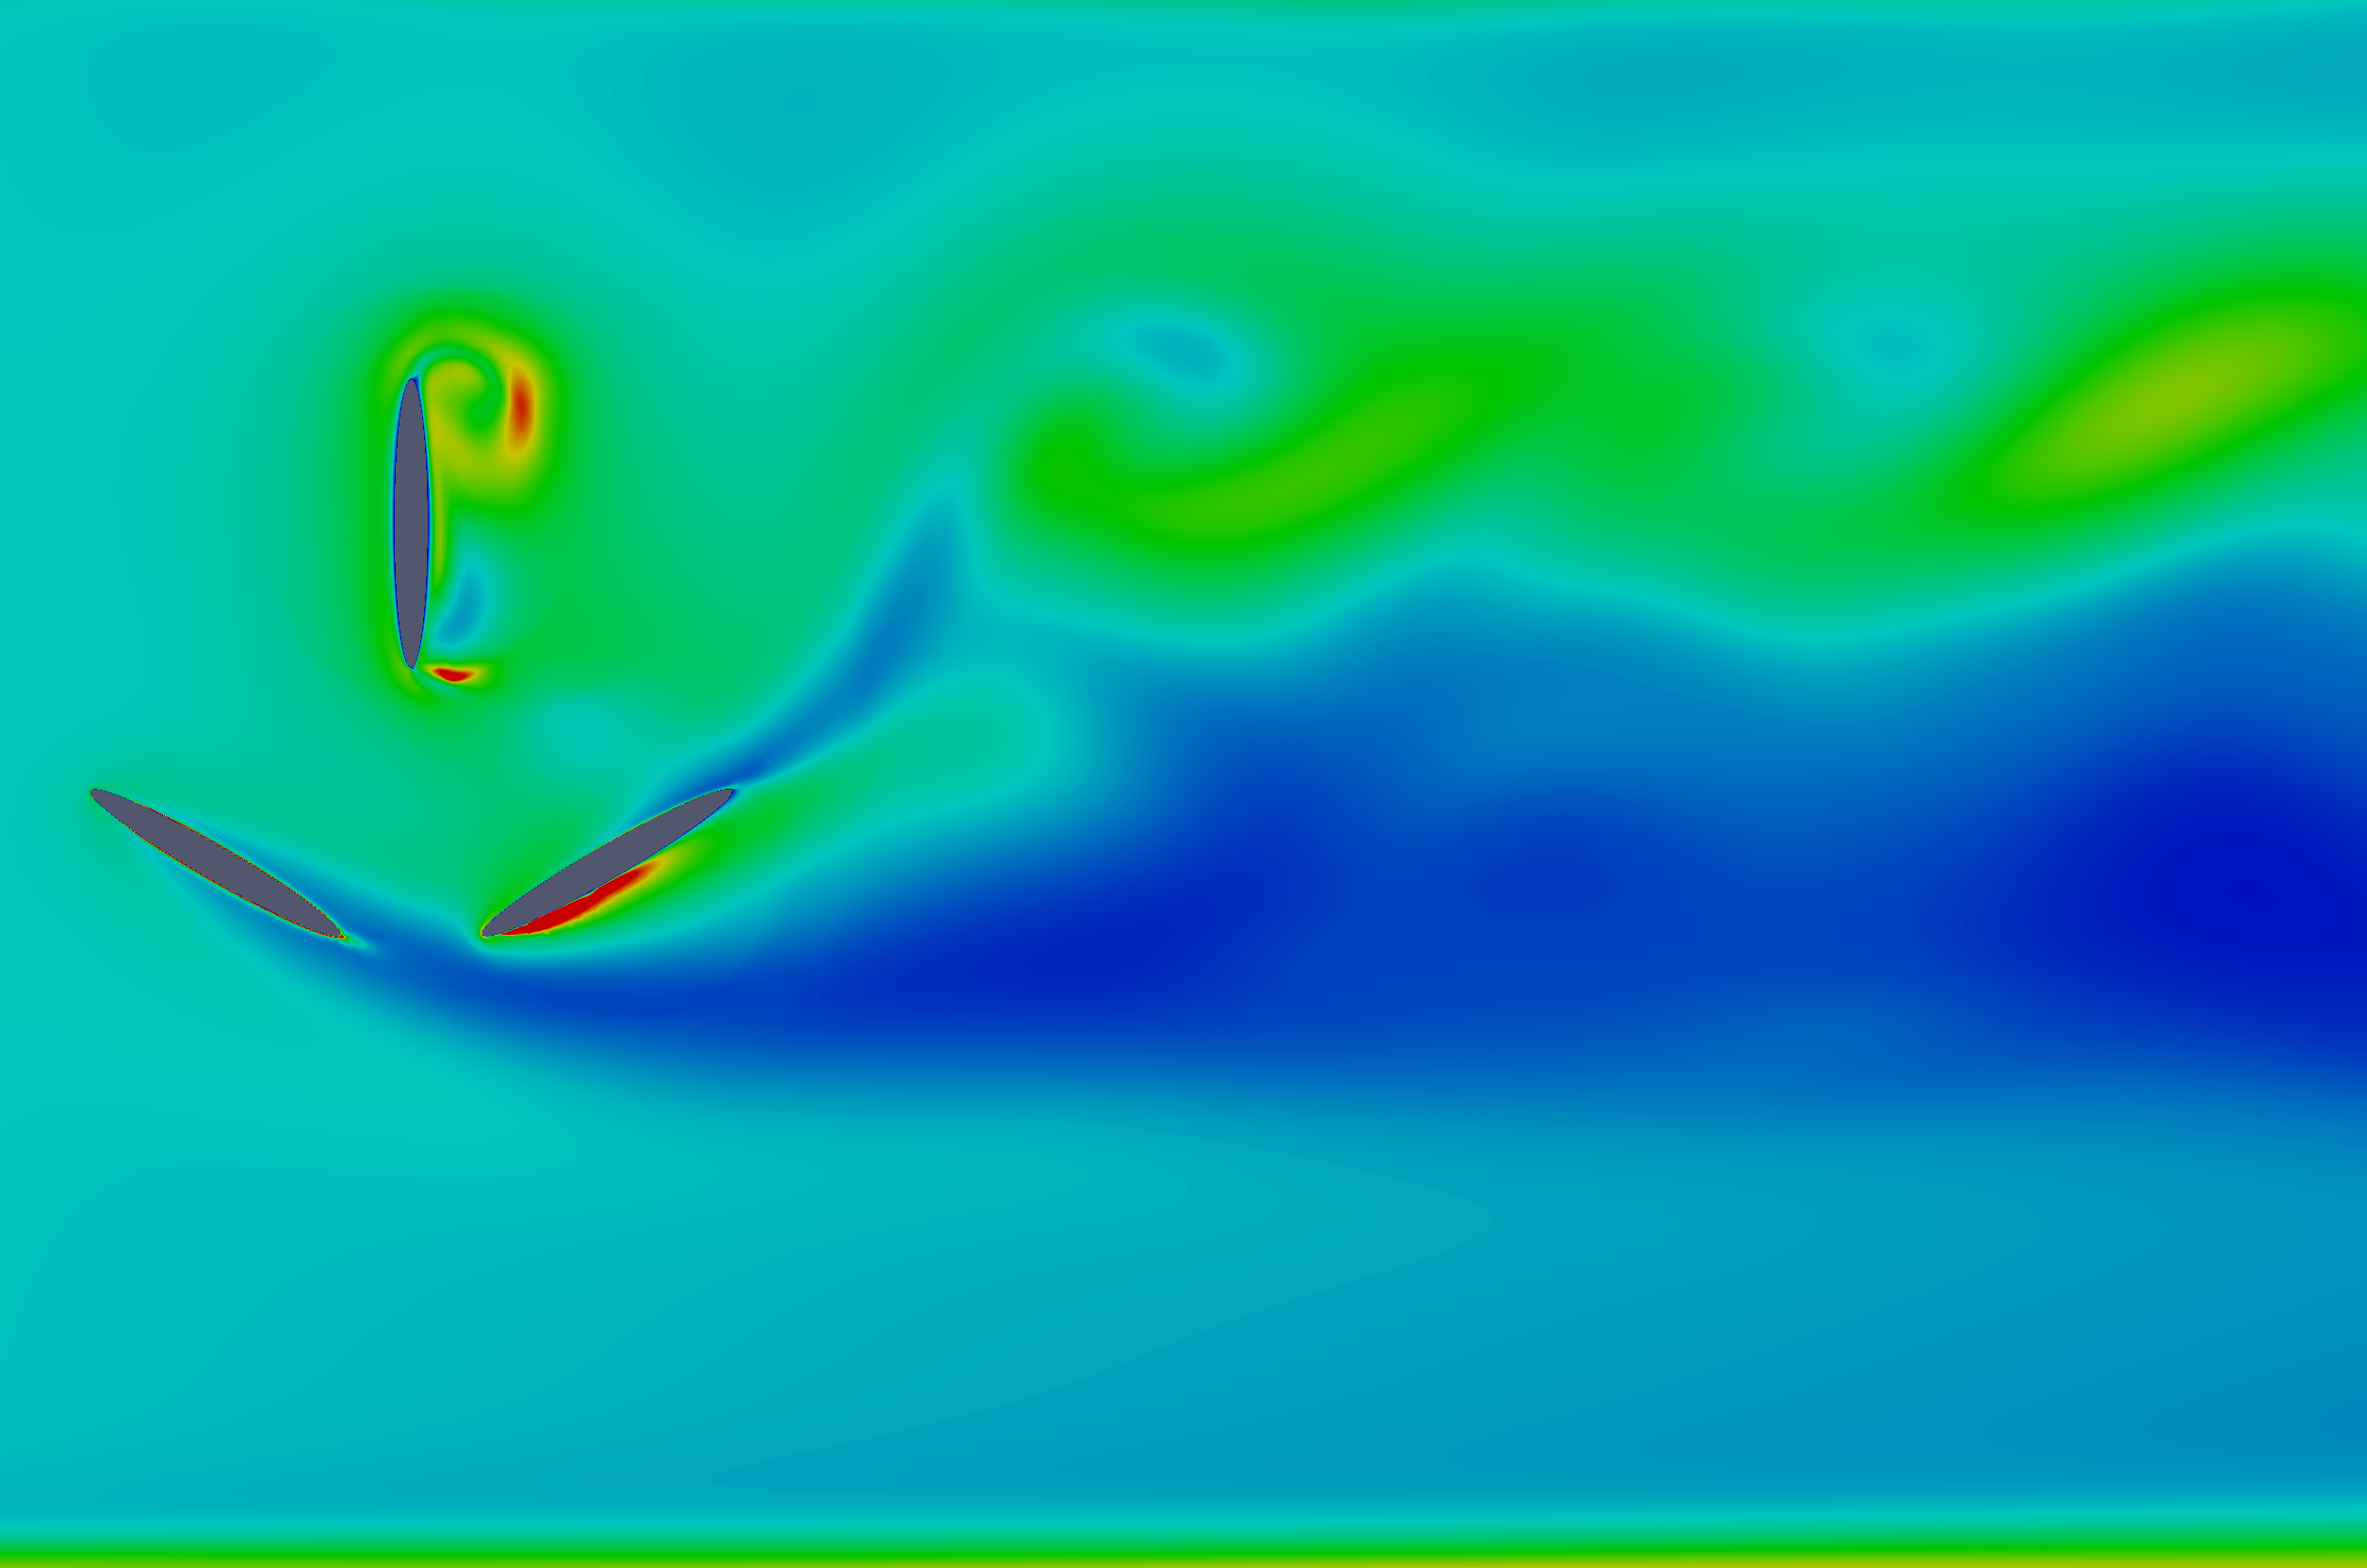
\includegraphics[width=\textwidth]{images/cover.png}
}
\date{}

% usefull for ltablex to split long tables in many pages
\keepXColumns

\DeclarePairedDelimiter\abs{\lvert}{\rvert}%

%\newcommand{\Fy}[1]{\text{F}_{y_{#1}}}

%\newcommand{\diameter}{\oslash}

%\newcommand{\todo}{\colorbox{cyan!60}{TODO}}

\renewcommand{\thesubsection}{\thesection.\arabic{subsection}}

\renewcommand{\arraystretch}{1.4}

\newcommand{\variable}[1]{\textcolor{blue}{#1}}

\newcommand{\paramtext}[1]{\textcolor{black!30!green}{#1}}

\newcommand{\terminal}[1]{\textcolor{black!30!cyan}{#1}}

\newcommand{\todo}{\colorbox{cyan!60}{TODO}}

\newcommand{\fakecaption}{%
  \vskip0.5\baselineskip
  \refstepcounter{table}%
  \tablename\ \thetable%
}

\makeindex

\begin{document}

\maketitle
\begin{center}
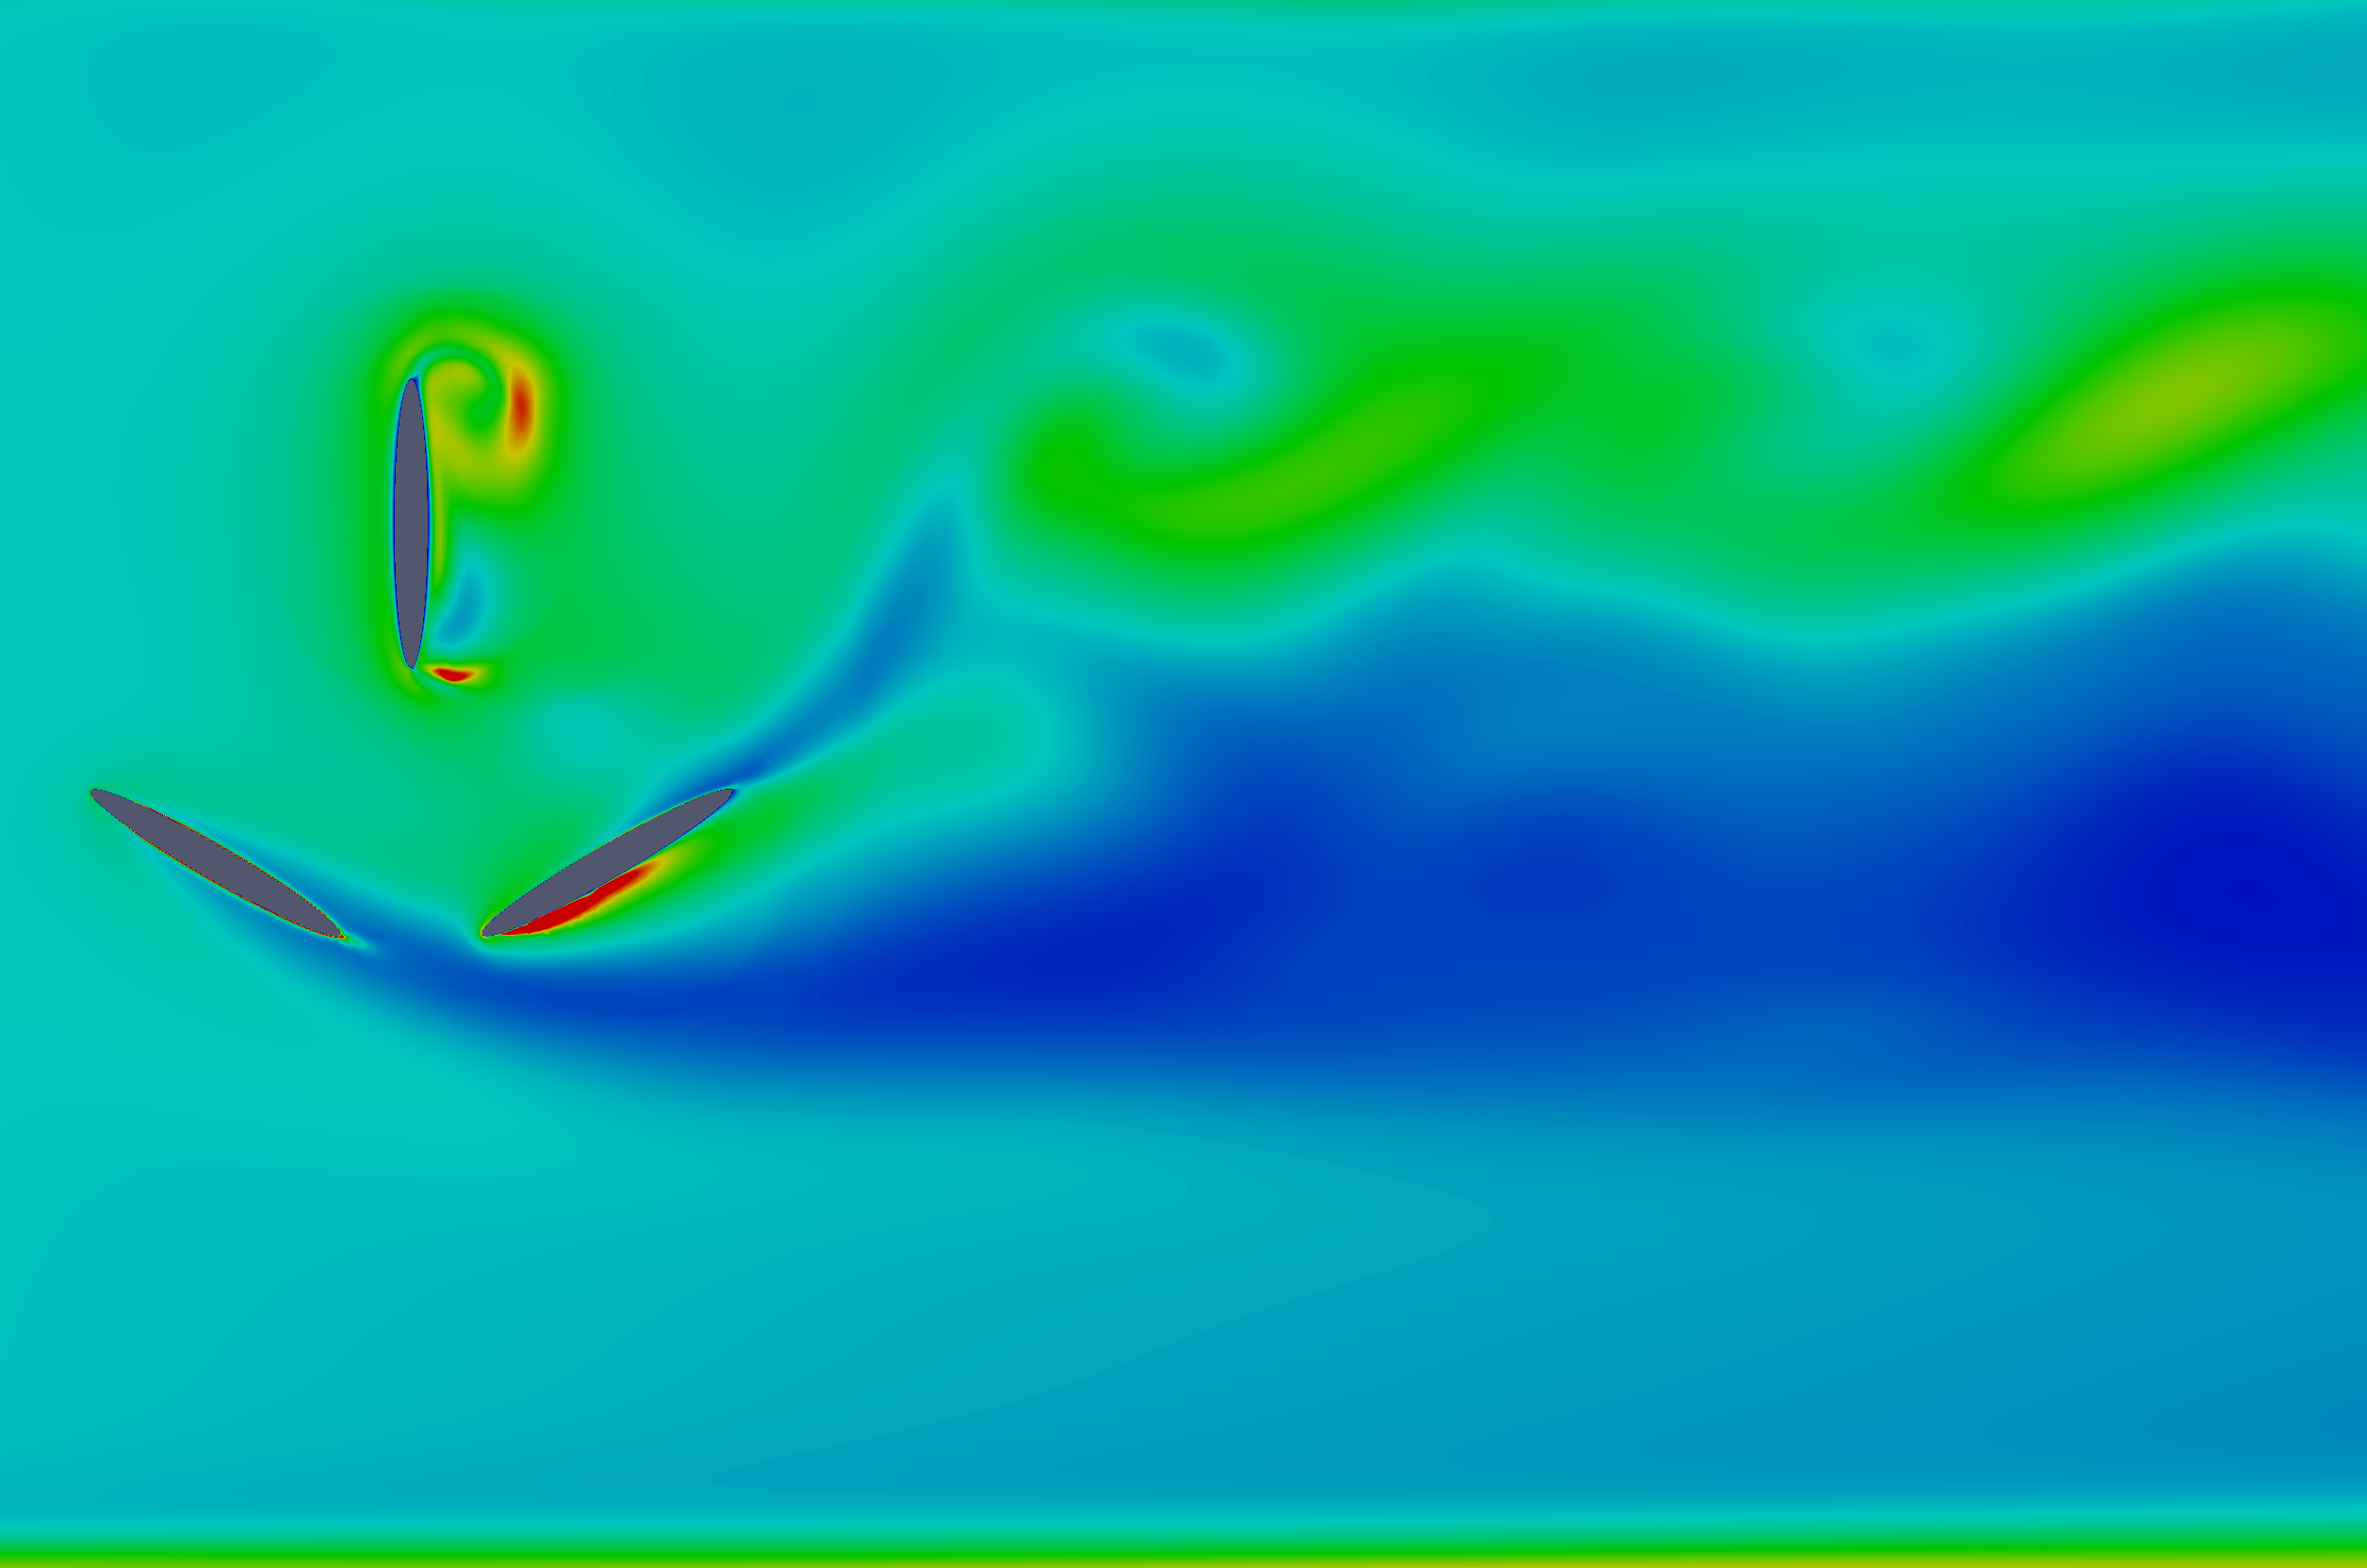
\includegraphics[width=\textwidth]{images/cover.png}
\end{center}

\newpage

\tableofcontents

\newpage

\section{Introduction}

\subsection{MRL Tidal Turbine Description}
The MRL Turbine is a hydraulic machine which is able to exploit the upcoming  water flow that is passing through the cross sectional area of the inlet of the machine. Momentum Reversal and Lift Tidal Turbine is a cross-
flow tidal-stream device which converts
 the energy of the water
flow into mechanical power.So the most advantageous locations in order to place this device are whatever kind of regular river with a smooth river bed or any sea/ocean areas which are subjected to relevant tidal phenomena.
The turbine is made up of three rotating blades and each blade is subjected to the combination of two rotating motions. A rotation $\omega_0$ along the machine axis  and a rotation omega1 around the blade individual axis with counter-rotating $\omega_0$ and $\omega_1$.

\begin{center}
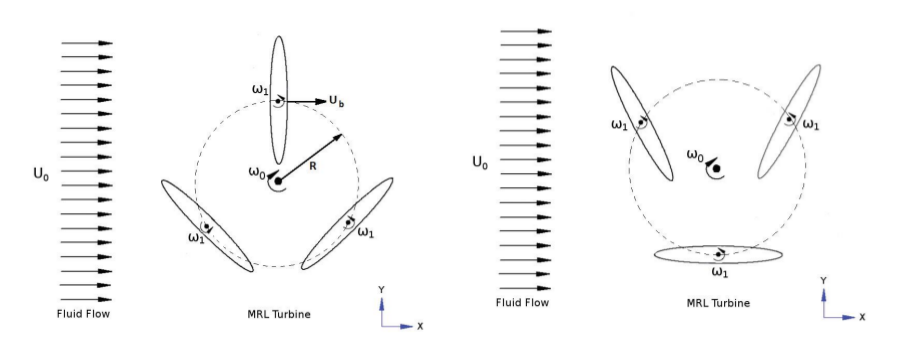
\includegraphics[width=0.8\textwidth]{images/flow.png} 
\end{center}

The flow-blade interaction leads to a drag force that is coming out while the blade is placed in the upper part of the circumferential path and a lift force on each blade located in the lower part of the path.
The resulting torque multplied by the rotating speed will give the generated power of the turbine which, in the end, is our final useful effect. The generated power per turbine is not really high (a few Watts) and this is the reason why the \emph{farm layout}  that Prof. Gavin Tabor showed us at the beginning of the course is used. Many little turbines are placed in a schematic and regular disposition in order to extract a higher power from the tidal stream.
Since from the first raw presentation of the machine we can realise that the mesh will have a relevant importance in the representation and validation of this complex rotating movement. We will deal with a rotating mesh which is progressivly refined closeto the blades, ending with the boundary layers when we are approaching the solid walls of the blades.


\subsection{The data}
The turbine is surrounded by an upcoming water flow set at 1 m/s constant along y axis. 
CAD files were provided by our professor and all the geometry parameters were known.
The in-class workflow has been divided into four little sub-tasks. 

The sub-tasks allowed us to start to get more familiar with the project work and understand the main issues met along the path with the help of the professors. The in-class project started with the raw mesh generation (blockMesh, snappyHexMesh), continued with the preparation of the rotating mesh(AMI files, baffles creation, merge and split procedure), movement of the mesh with the provided motion laws  (real turbine rotation, gif rendering) and finally the set up, running and post processing of the simulation.

\section{In-class work}
\paragraph{In-class workflow}\mbox{}\\
The in-class workflow has been divided into four little sub-tasks. The sub-tasks allowed us to start to get more familiar with the project work and understand the main issues met along the path with the help of the professors. The in-class project started with the raw mesh generation (blockMesh, snappyHexMesh), continued with the preparation of the rotating mesh(AMI files, baffles creation, merge and split procedure), movement of the mesh with the provided motion laws  (real turbine rotation, gif rendering) and finally the set up, running and post processing of the simulation.

\paragraph{Mesh generation}\mbox{}\\
One of the most challenging section of the in-class project was the generation of the raw turbine domain mesh. We have used many different openFoam comands in order to build a complete and exhaustive mesh that must be suitable for the hydraulic problem characteristics.
\\ 
Let's start to present the overall mesh work-flow with all the brief steps evaluation.
\\
\begin{itemize}
\item The scaling of the dimensions and geometry parameters coming from the stl files from millimiters to meters in order to perform correst calculations in the openFoam environment;

\item BlockMesh and SnappyHexMesh for each of the three blades. At this point castellated, snapped and layered mesh have been realized for each blade and we have to join all together;

\item Merging procedure in order to have one complete mesh and the copy of the mesh inside our main environment of the project. We have decided to oparate in this way in order to have a better comunication level in terms of interpolation values among mesh sub-domains. In this way the neighboring cells of different sub-domain are well oriented and aligned. The result is an improvement on the mesh quality controls as non-orthogonality index and skewness coefficient  because we have parallel disposition of cells and they appear as concentric refined layers;

\item Mesh extrusion with the thickness of the 2D domain already given as a geometry parameter equal to the blade width);

\item Wall layer refinement;

\item The first mesh is the 40$\times$120 mesh where the couple of numbers indicates the number of squared and regular cells that are disposed in the y and x direction respectively in the blockMeshDict definition.  
\end{itemize}

Since we deal quite often with different mesh size, in particular during the mesh senitivity analysis, we will call mesh $i$ the mesh with $i$ cells in the y direction, and the cells in the x direction are such a number that let to have squared cells, in order to make the comparison easier and faster to understand.

\paragraph{In-class simulation}\mbox{}\\
In the final part of the in-class project we performed the set up and run of the first raw simulation.
To do so, we have to manage with the boundary conditions of the problem, the turbolence modeling and the numeric schemes. All thease macro-section of the simulation were assigned a priori and the last part of our work is to play with all these parameters and try to understand the influence of each singular changing in the set up on the final result that the turbine must provide.

For the first setup we use the simpler $k\!-\!\varepsilon$ turbolence model respect to more appropriate $k\!-\!\omega \, \text{SST}$.

\subsection{Boundary conditions}
Boundary conditions are referred to the water stream velocity that is investing the machine, the pressure of the water in the stream channel, k, w and nut values.

Our main interest is to focus the first two boundary conditions so velocity and pressure, since the other are maily taken as the default condition for the respective turbolence model.

\paragraph{Patches}\mbox{}\\
Boundary condition are defied over patches so it is important to define that.
\begin{itemize}
\item \emph{Inlet Section} is that from which water comes into the domain moving toward the x direction;
\item \emph{Outlet Section} is where water comes out from the domain;
\item \emph{Front and back faces} are always set to empty since we are dealing with a 2D problem;
\item \emph{Lower wall} is a physical wall that limit the flow;
\item \emph{Upper wall} is a free surface where the flow can slip;
\item \emph{Blades} are physical surfaces that moves inside the domain;
\item \emph{Ami interfaces} are internal patches that allow the communication between moving adiacent cells. All the quantities are set as CyclicAmi.
\end{itemize}


\paragraph{Velocity U}
\begin{itemize}
\item \textbf{Internal field} is uniform at the beginning and it is set to $1\ms$ in the x direction even if in class we have set inlet velocity to $1\ms$ and internal field inited to $0\ms$. We take this decision to make the transition phase faster to limit the simulation time. We are actually interested only in staeady state power so limit the transition let to reduce computational time;
\item \emph{Inlet Section} velocity is fixed to $1\ms$ during all the simulation; 
\item \emph{Outlet Section} velocity is unknown so we have to set it to ZeroGradient boundary condition;
\item \emph{Upper wall} velocity is set to Slip since the fluid can flow in the free stream;
\item \emph{Lower wall} velocity is set to NoSlip which is equivalent to fix the value to zero;
\item \emph{Blades} velocity is set to MovingWallVelocity which is equivalent to NoSlip for moving bodies;
\end{itemize}

\paragraph{Pressure $p$}
\begin{itemize}
\item \textbf{Internal field} is uniform at the beginning and it is set to $0$. 
OpenFoam for incompressible cases works with pressure normalized respect to density. 
Moreover it can manage relative pressures. 
So the value that we set is relative $0 \,\text{bar} \cdot \text{m}^3 / \kg = \m / \s^2$.
\item \emph{Inlet Section} pressure distribution unknown so we set to ZeroGradient; 
\item \emph{Outlet Section} is set to atmospheric ($0 \m / \s^2$) since we assume to be sufficiently far from the blades that pressure is constant;
\item \emph{Upper wall} pressure is set to atmospheric since it is free stream;
\item \emph{Lower wall} pressure is set to ZeroGradient since boundary layer are isobar;
\item \emph{Blades} pressure is set to ZeroGradient since boundary layer are isobar;
\end{itemize}

\paragraph{Turbolent quantities $k$, $\varepsilon$, $\omega$, $\nu_T$}\mbox{}\\
For what that concern the boundary conditions of the turbolence quantity we apply default settings.
We will discuss instead a modification of the value of initialization of that quantity to speed up as much as possible the convergence to a steady state condition.

\paragraph{Solver}\mbox{}\\
The solver applied in the class session is pimpleDyMFoam in PISO mode with one outer corrector, two inner correctors and no non orthogonal correctors. This solver is responsible not only for the solution of the system of differential equation, but also for the movement of the mesh at each time step. 

\section{Mesh sensitivity Analysis}
With the mesh sensitivity analysis second part of the report starts. Here we are interested to find the proper value of parameters that let to have the best simulation as possible.

The first and probably the mos significant operation is the mesh sensitivity analysis.
\\
The aim is to find a tradeoff between \emph{accuracy} and \emph{computational cost}. 

The expected improvement into the quantities of interest decreases with the increase of the number of cells.

There is a point beyond which the improvement becomes really negligible and we encounter a plateau; beyond that it not worth the increate in computational time. 

Our sensitivity analysis includes 6 different simulation:
\begin{itemize}
\item mesh 20
\item mesh 40
\item mesh 60
\item mesh 80
\item mesh 120
\item mesh 160
\end{itemize}

The choise of the level of vertical cells depends on the need to exploit 3 different steps in which the number of cells becomes 4 times bigger. Actually we pass from approximately 10000 cells of the mesh 20 to 40000 cells of the mesh 80 finally to around 160000 cells of the mesh 160. 
The ratio four explains the necessity to double the cells number in each of the relevant dimensions of our 2D problem.

Despite the fact that the power generated is not the best indicator possible for highliting sensitivity behaviour it is instead the most relevant output parameter of our simulation.
Beside that we put also the total pressure drop that is a measure of the losses due to the turbine.
To compute the drop we consider the averate of the total pressure at the inlet and at the outlet both calculated at the end of the simulation.

During the choice of the mesh we have expoited two different possibilities:
\begin{itemize}
\item with a refinement region around the blades;
\item without a refinement region.
\end{itemize}
In both cases the same layer were present.
What we have noticed is that the results in terms of power were slighlty different, so we have decided to perform mesh sensitivity analysis with both the meshes.

\begin{figure}
\subfigure[Mesh 120 without refinement region]{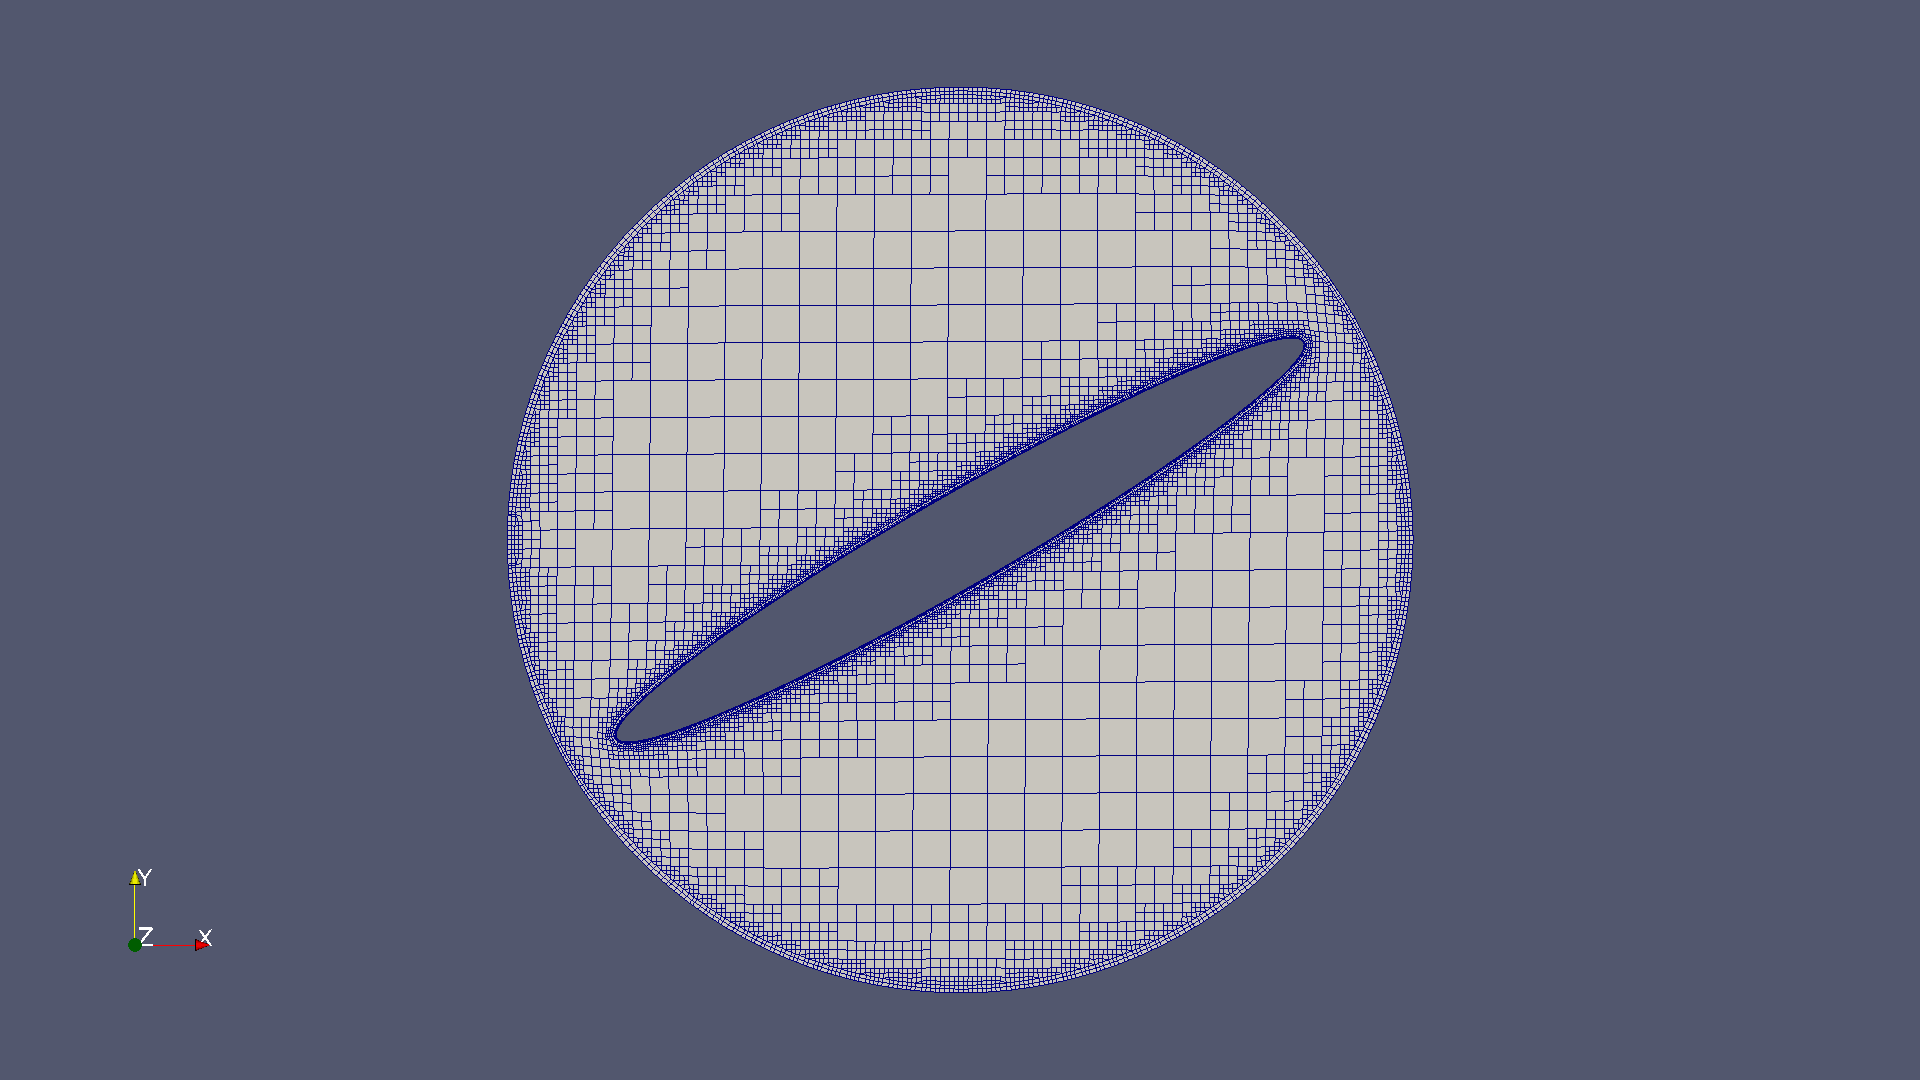
\includegraphics[width=8.5cm]{images/meshsensitivity/mesh120-blade0-noregion.png}}
\hfill
\subfigure[Mesh 120 with refinement region]{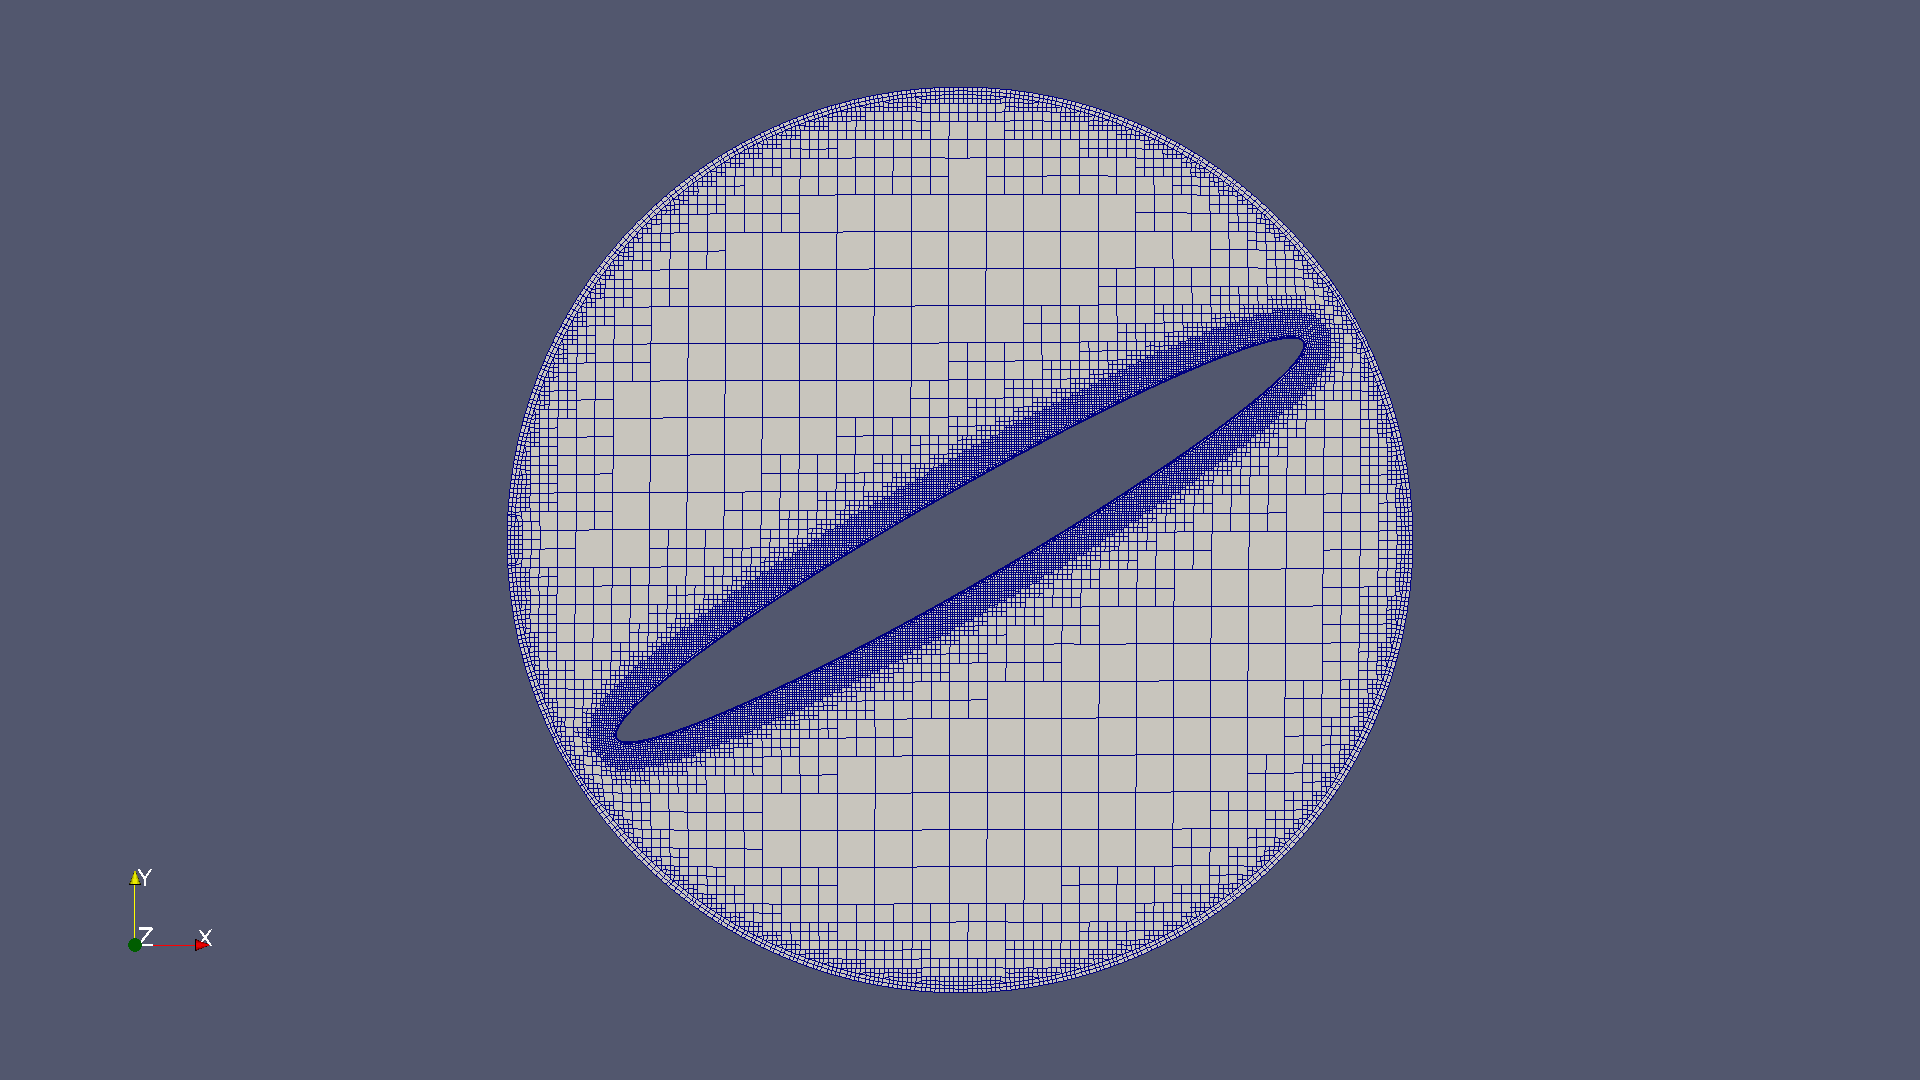
\includegraphics[width=8.5cm]{images/meshsensitivity/mesh120-blade0-region.png}}
\caption{Comparison between meshes with and without refinement.}
\end{figure}

\begin{figure}
\subfigure[Mesh 20 without refinement region]{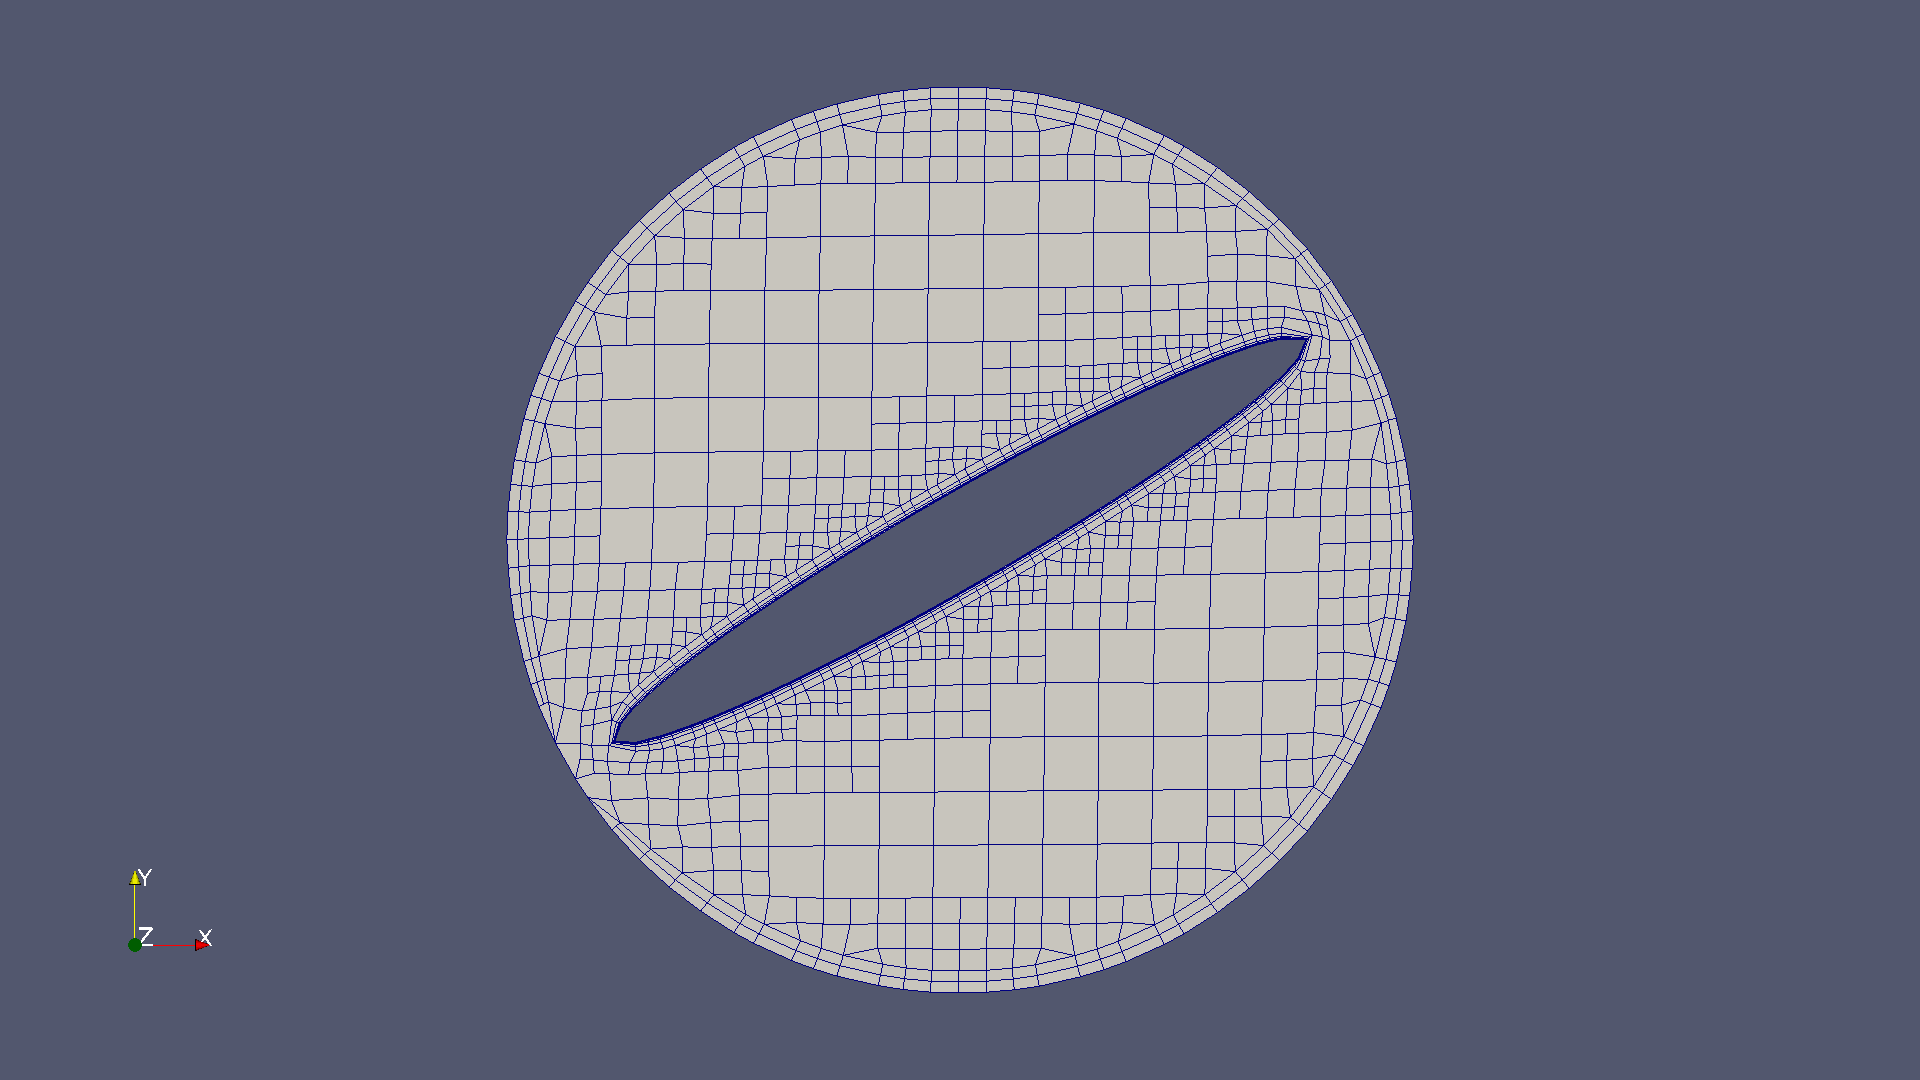
\includegraphics[width=8.5cm]{images/meshsensitivity/mesh20-blade0-noregion.png}}
\hfill
\subfigure[Mesh 40 without refinement region]{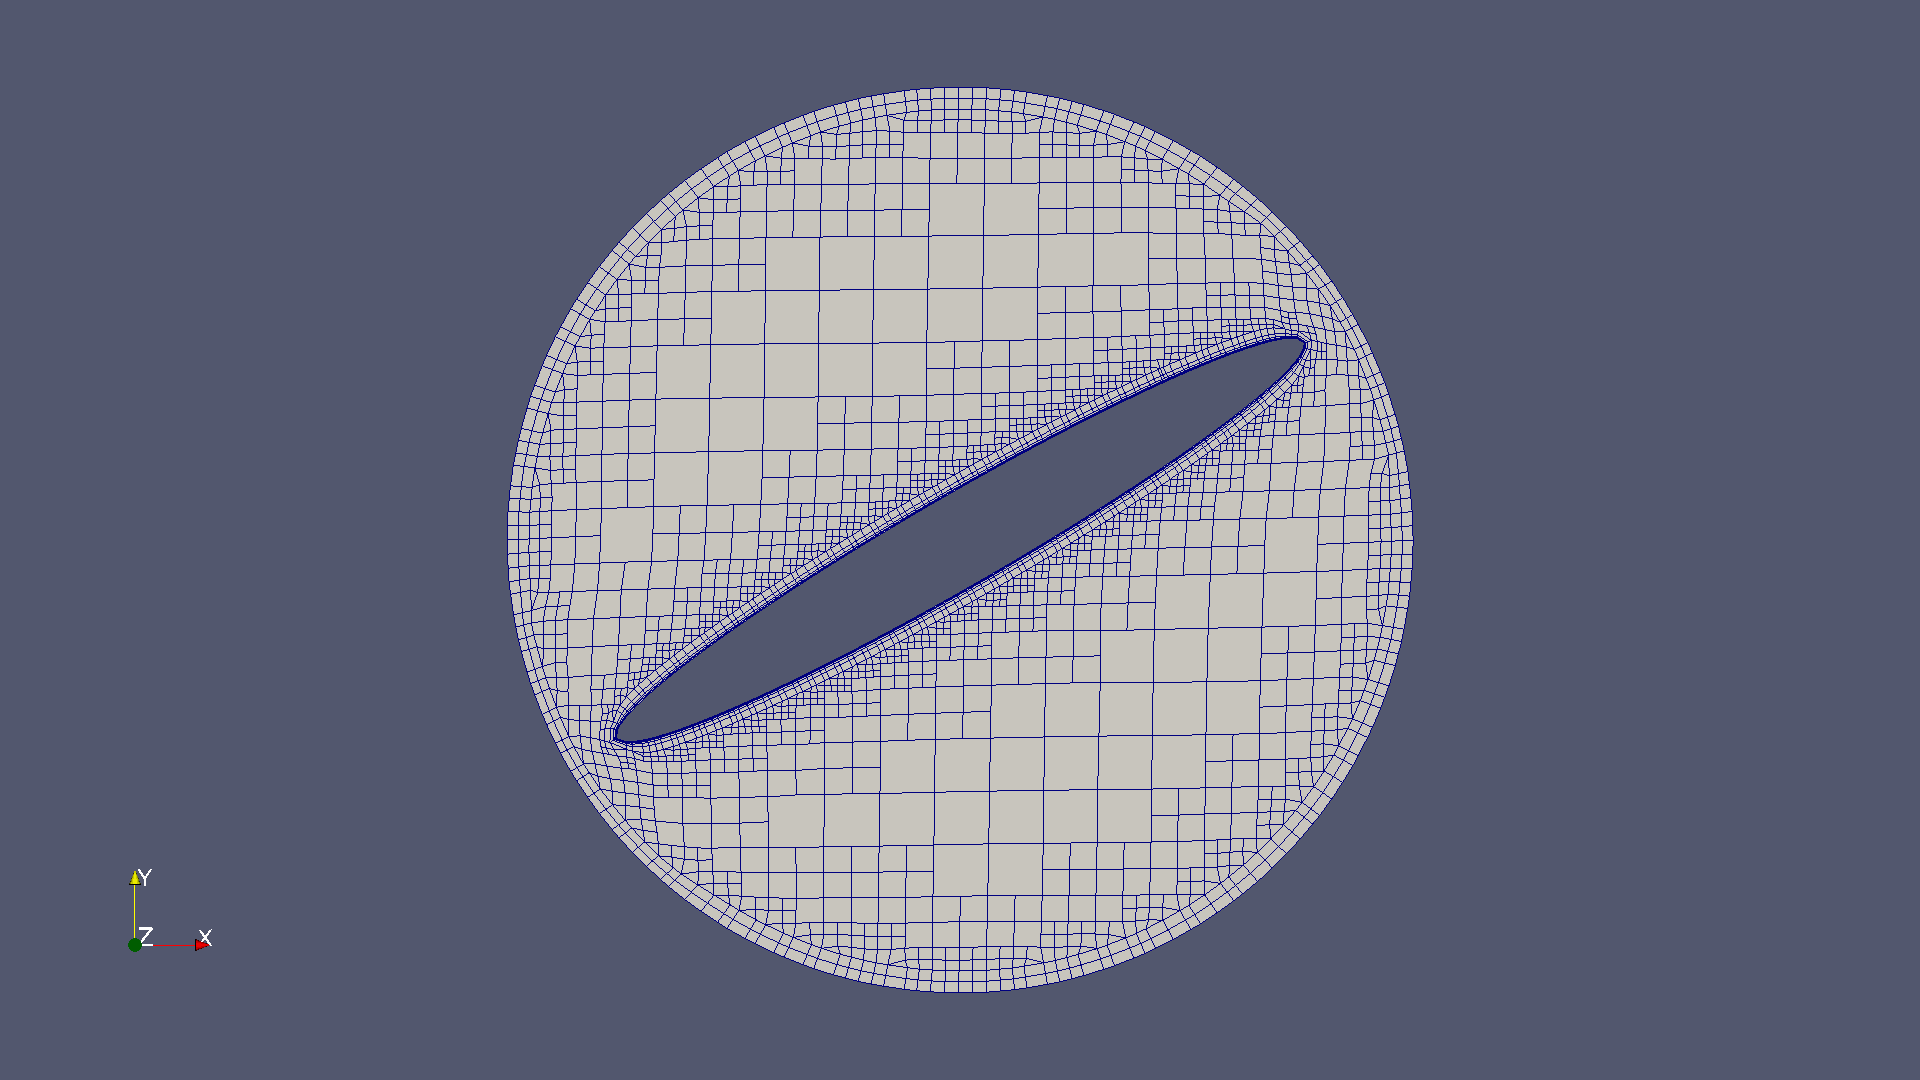
\includegraphics[width=8.5cm]{images/meshsensitivity/mesh40-blade0-noregion.png}}
\subfigure[Mesh 60 without refinement region]{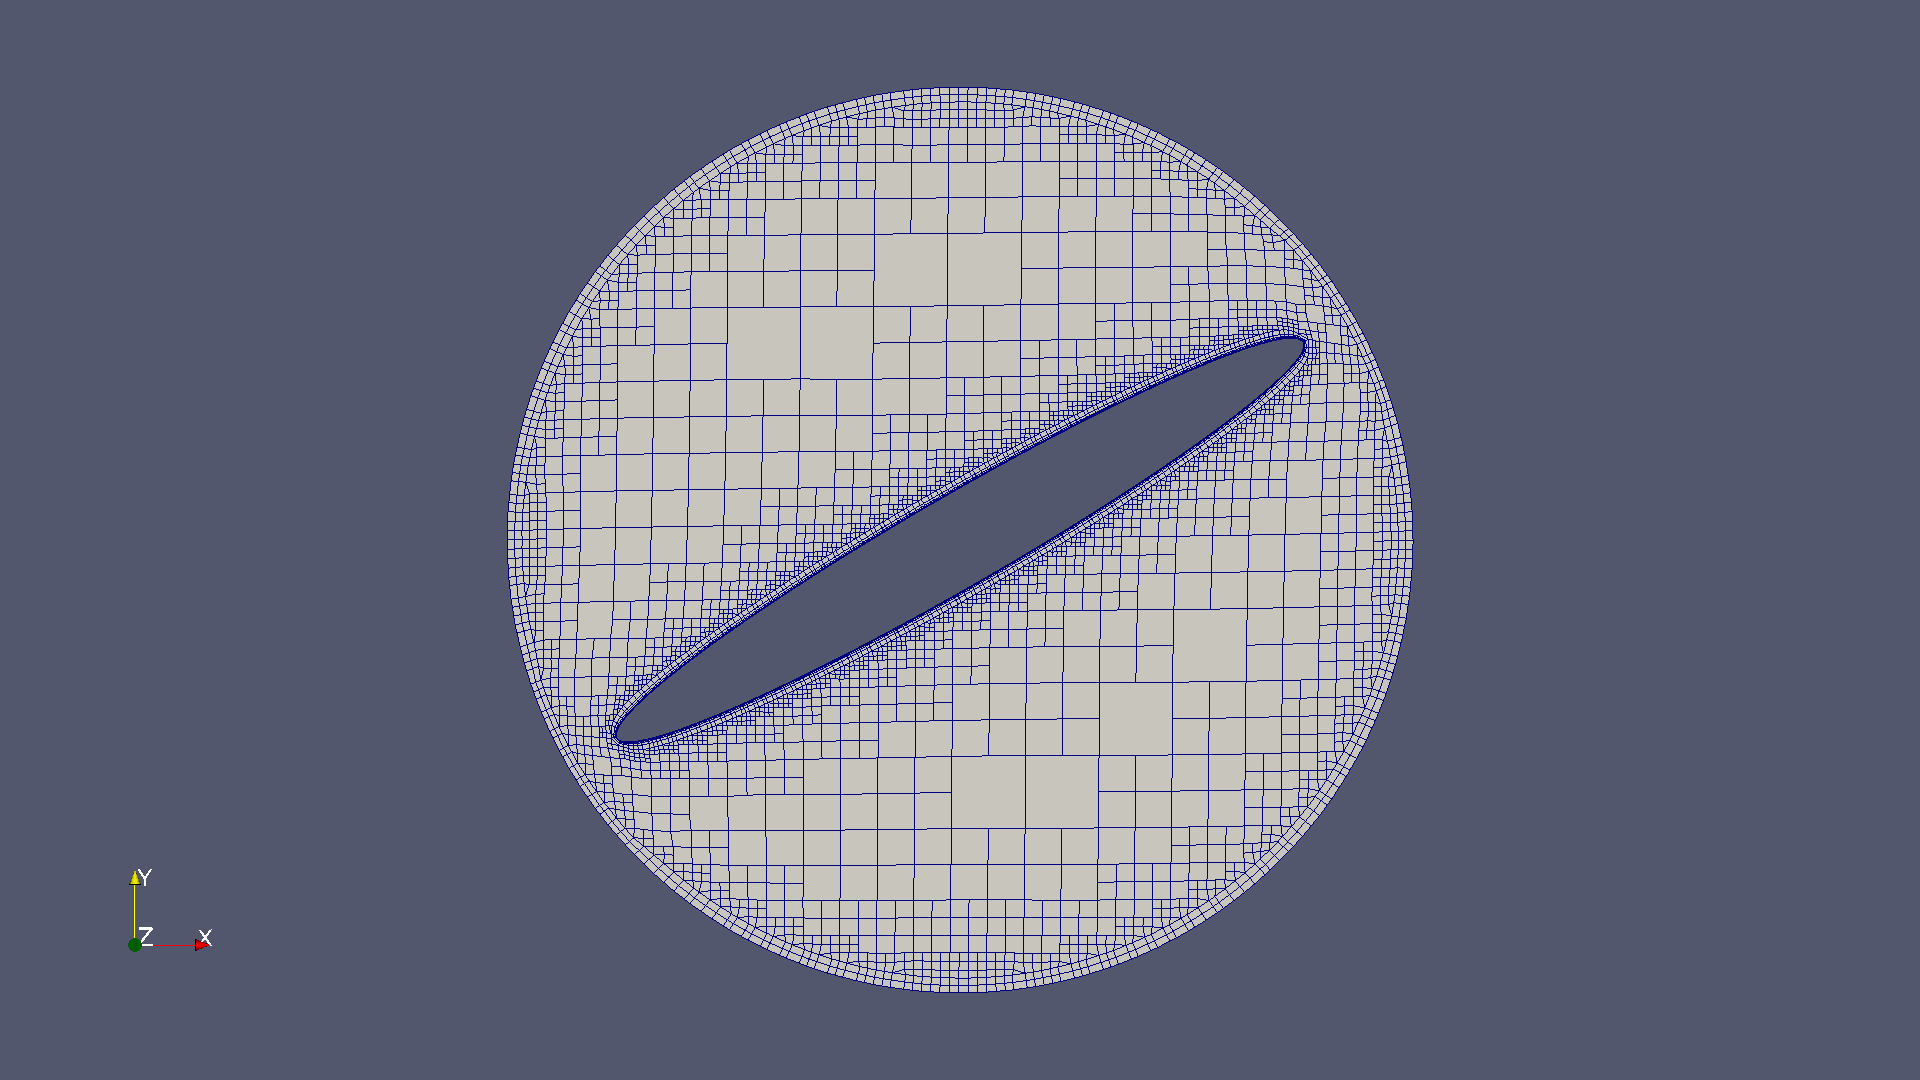
\includegraphics[width=8.5cm]{images/meshsensitivity/mesh60-blade0-noregion.png}}
\hfill
\subfigure[Mesh 80 without refinement region]{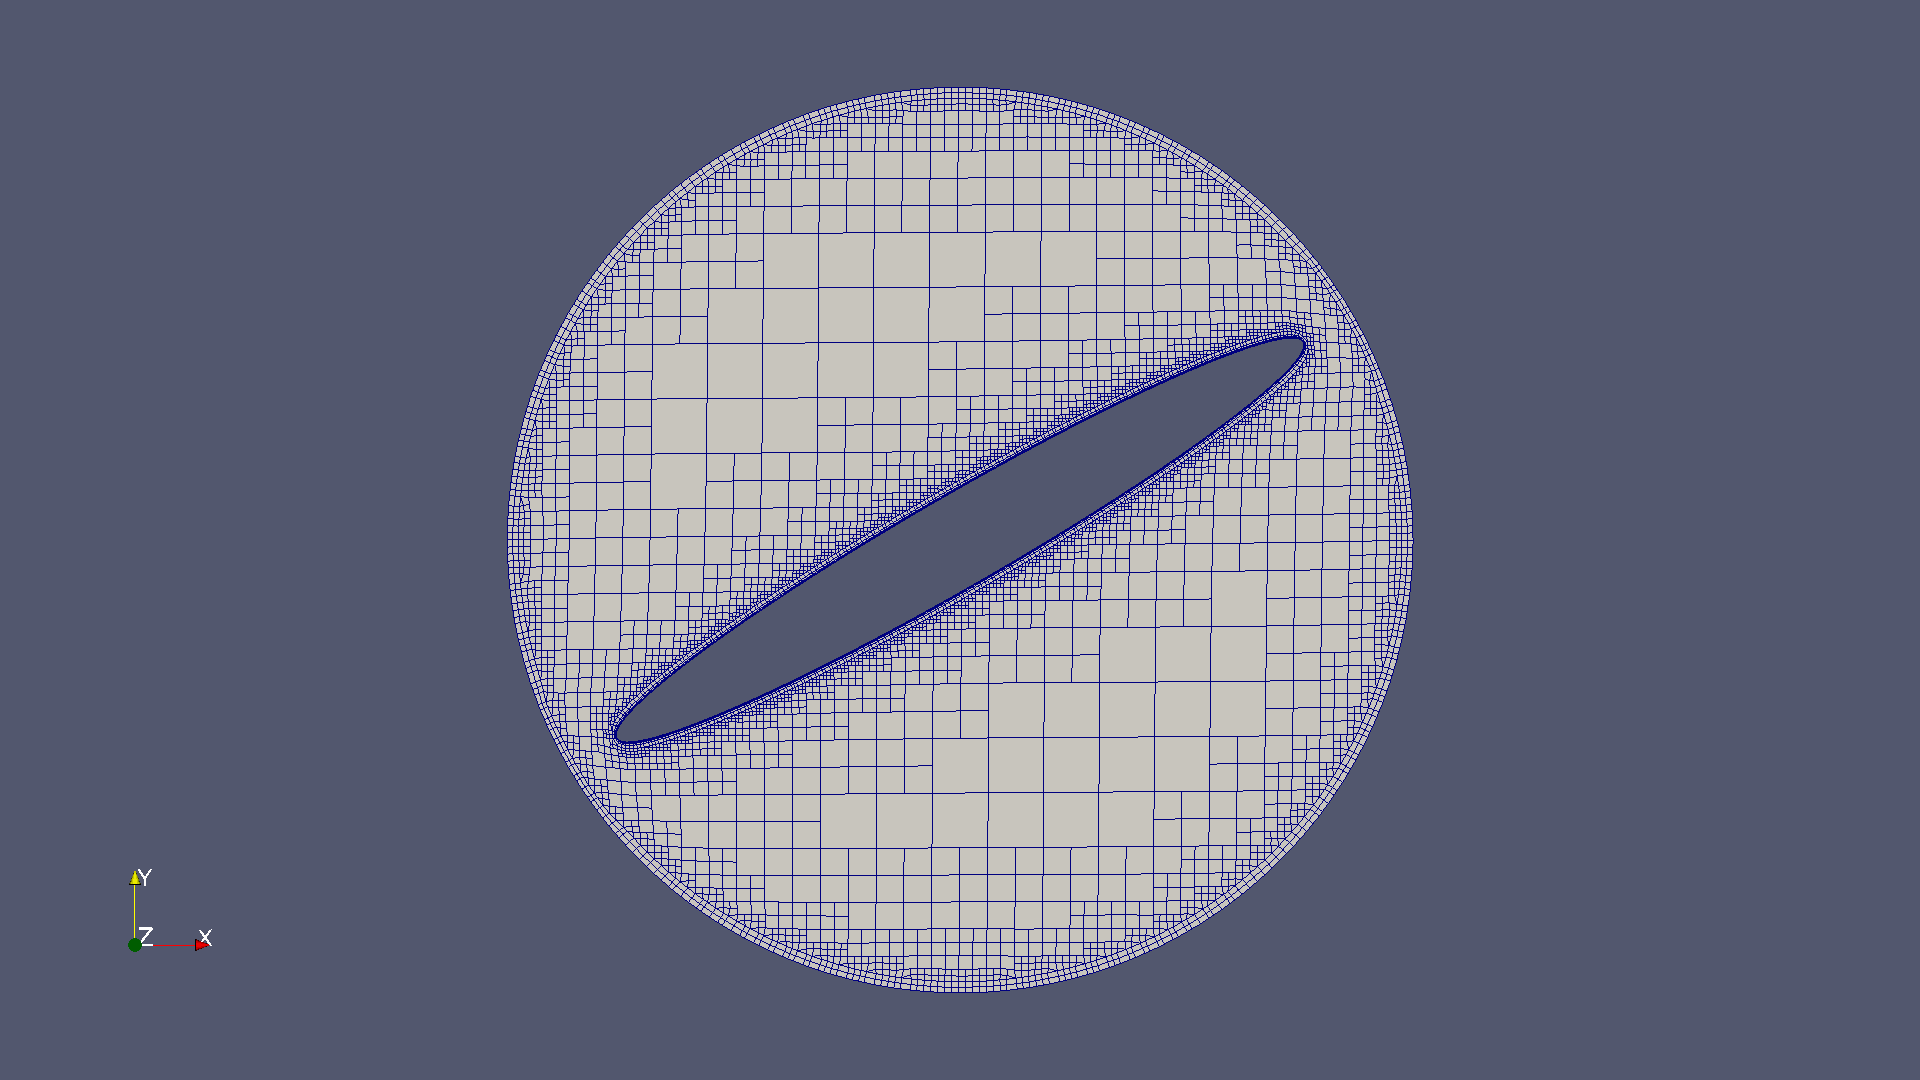
\includegraphics[width=8.5cm]{images/meshsensitivity/mesh80-blade0-noregion.png}}
\subfigure[Mesh 120 without refinement region]{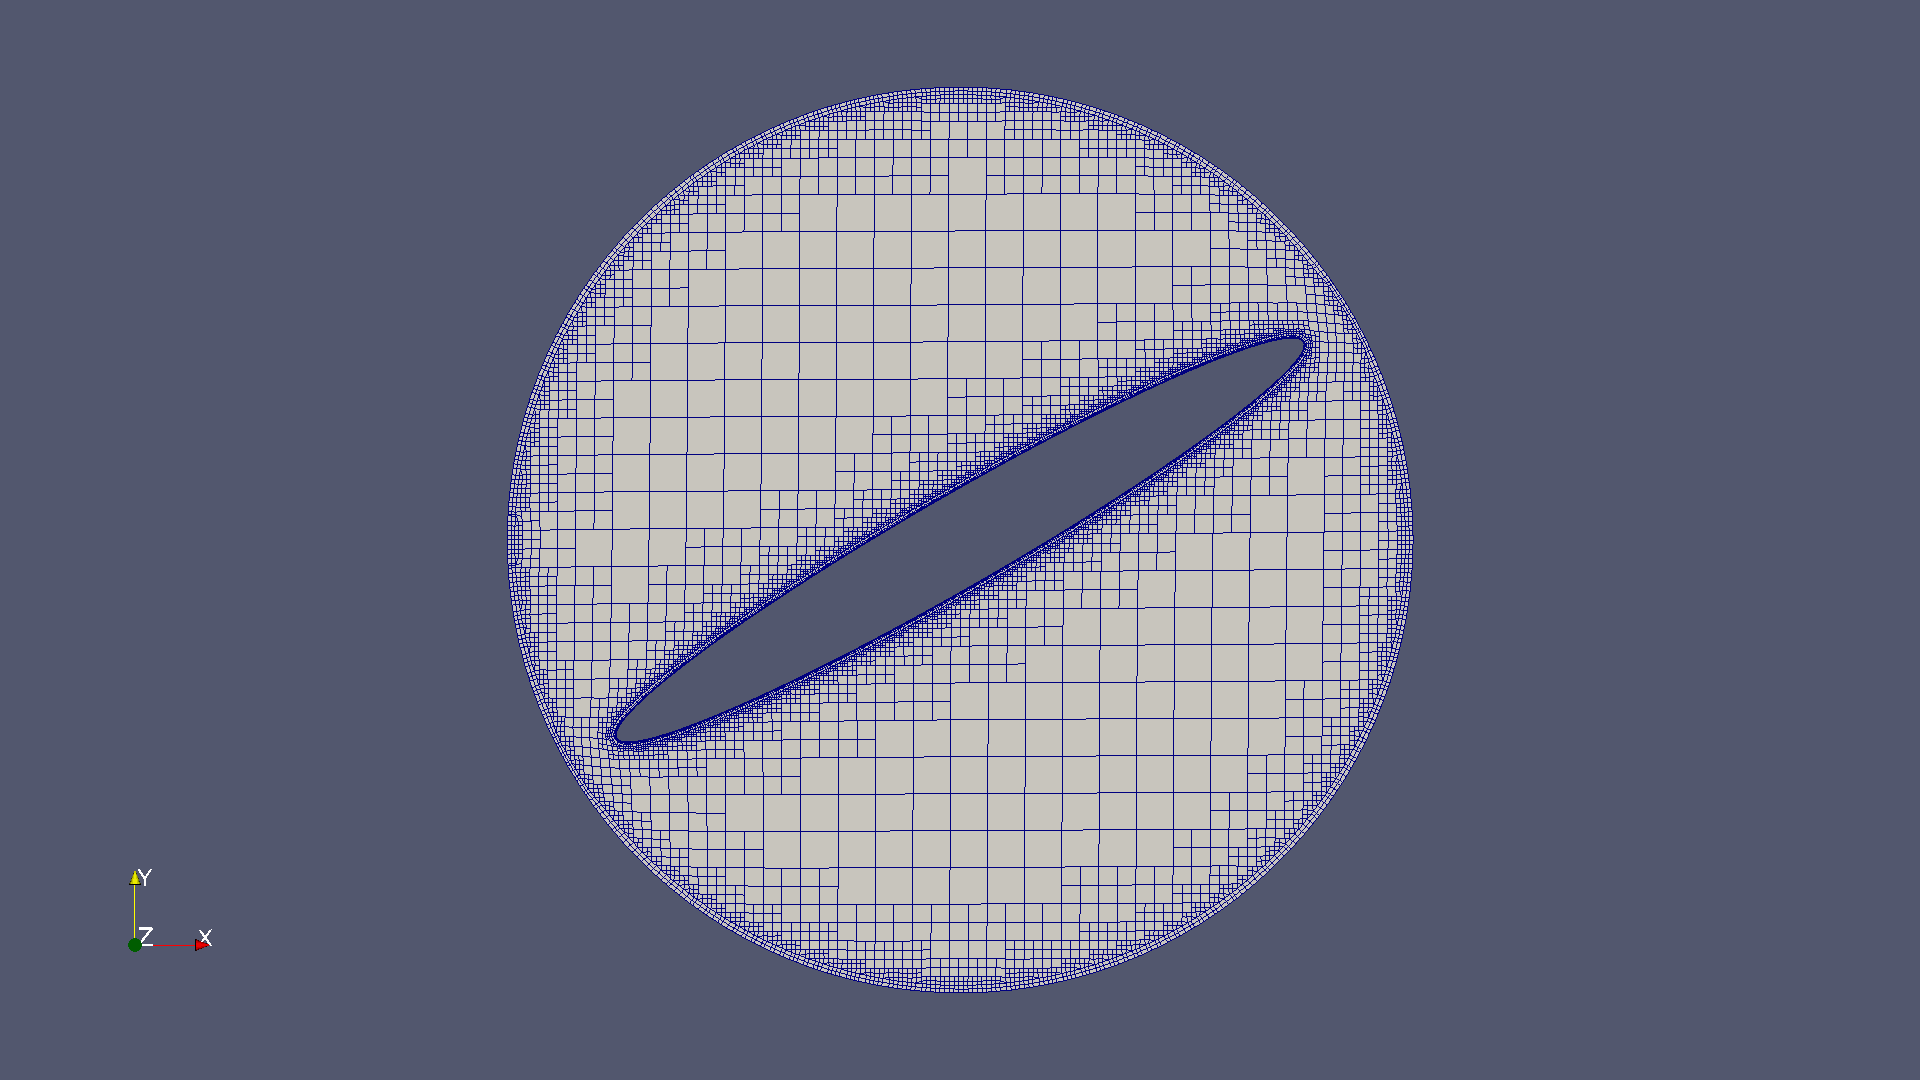
\includegraphics[width=8.5cm]{images/meshsensitivity/mesh120-blade0-noregion.png}}
\hfill
\subfigure[Mesh 160 without refinement region]{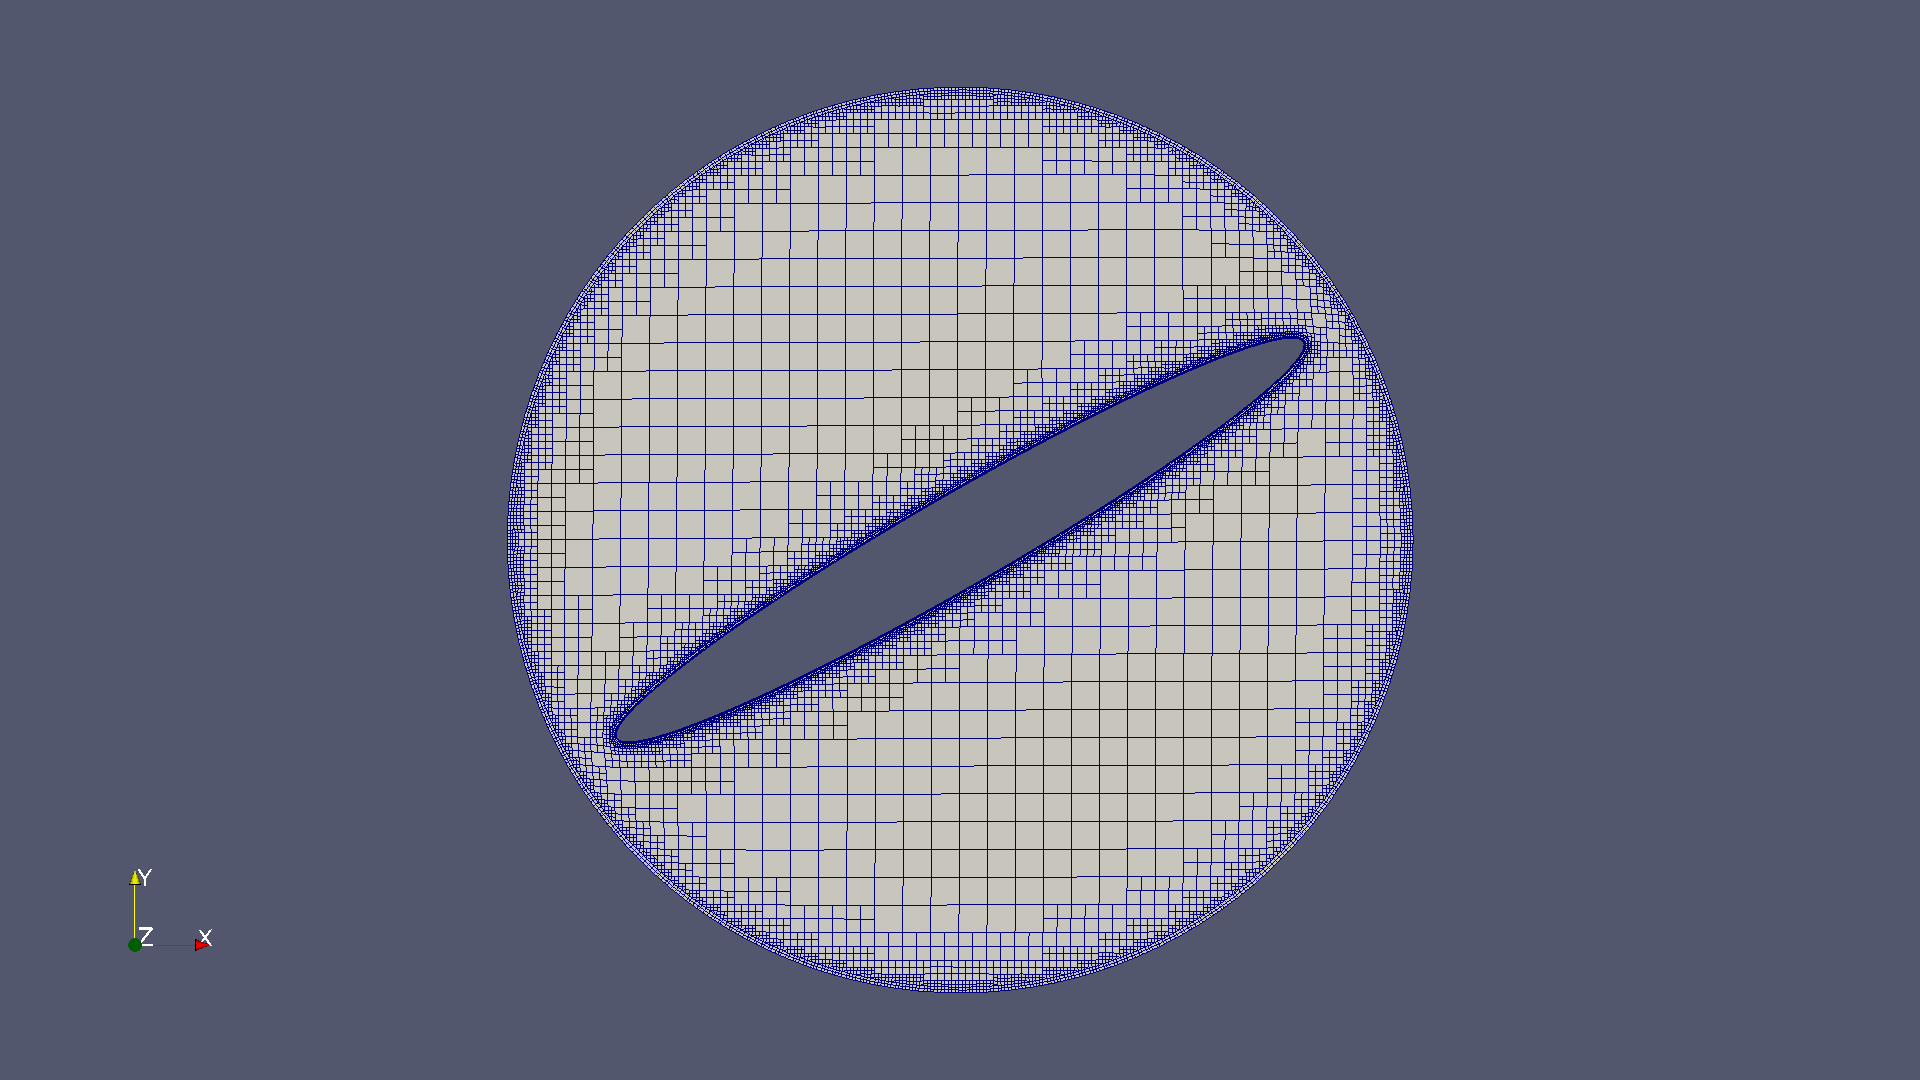
\includegraphics[width=8.5cm]{images/meshsensitivity/mesh160-blade0-noregion.png}}
\caption{Comparison between different mesh sizes.}
\label{fig:noregion-allmeshes}
\end{figure}

Given the mesh in figure \ref{fig:noregion-allmeshes} we have performed the simulation and extracted both power and total pressure drop.

\paragraph{Number of cells}\mbox{}\\
In table \ref{table:cellsnumber} we can find the cells number of the varius simulations.
\begin{table}[H]
\centering
%\begin{tabular}{@{}lrr@{}}
\begin{tabular}{lrr}
\toprule
         & Without region & With region \\ \midrule
Mesh 20  & 10328          & 9696        \\
Mesh 40  & 24066          & 24021       \\
Mesh 60  & 40462          & 42508       \\
Mesh 80  & 58877          & 64293       \\
Mesh 120 & 103384         & 120614      \\
Mesh 160 & 156791         & 160547      \\ \bottomrule
\end{tabular}
\fakecaption
\label{table:cellsnumber}
\end{table}

\paragraph{Power:} for the power we have make the simulations run for 4 periods from 0 to 2.4 seconds and then we have taken the average of the power over the last turn, between 1.8 and 2.4 seconds.
We have done this since we have assumed that the last revolution was the best indicator of the steady state behaviur of the turbine.


\begin{figure}[htbp]
\centering
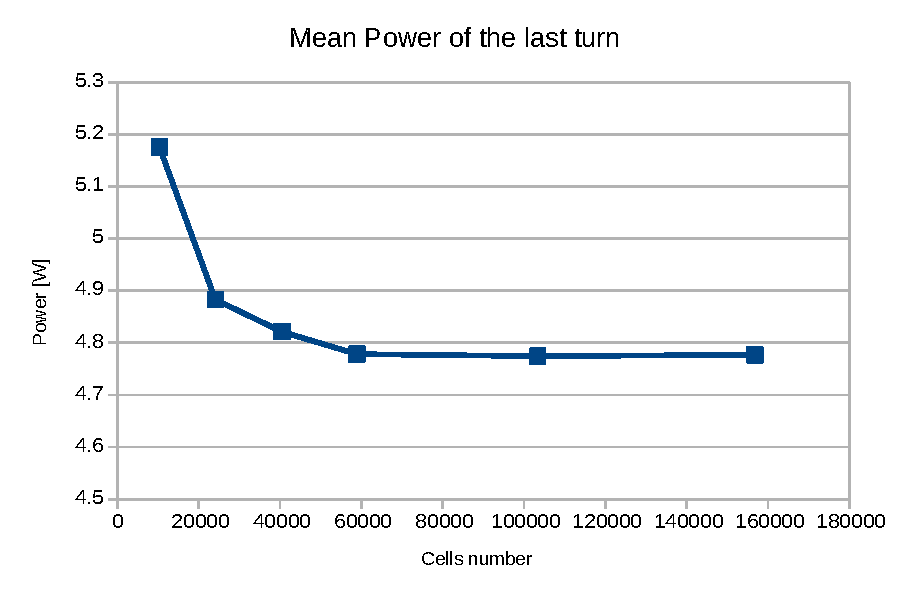
\includegraphics[width=8.5cm]{images/meshsensitivity/power-noregion} 
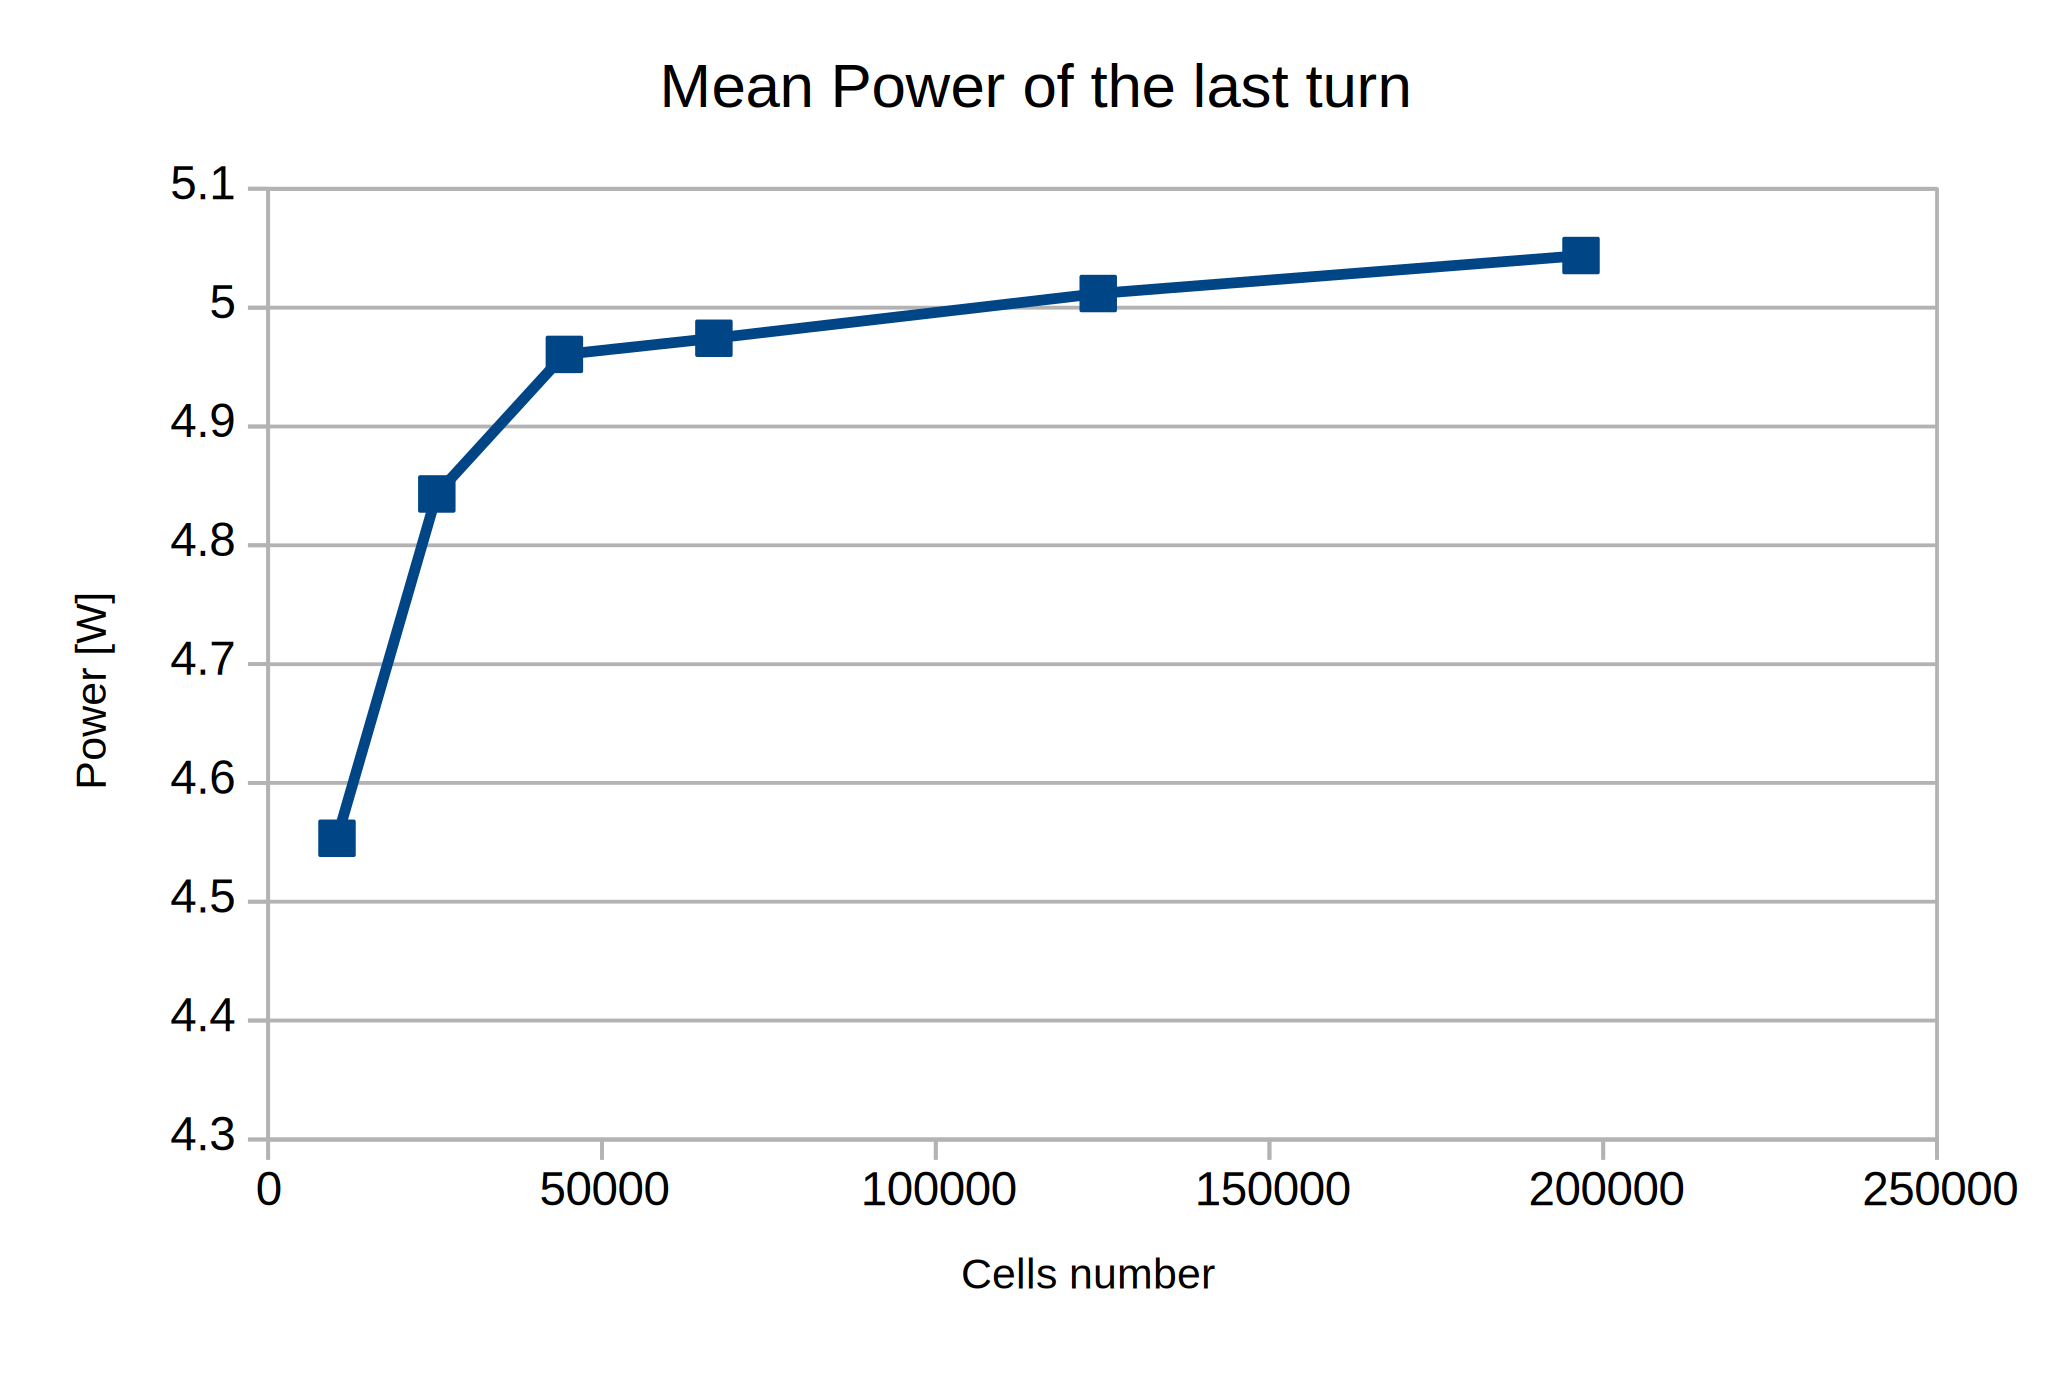
\includegraphics[width=8.5cm]{images/meshsensitivity/power-region} 
\caption{Average power in time between 1.8 and 2.4 seconds}
\label{fig:meshsensityvity-power}
\end{figure}

As we can see in figure \ref{fig:meshsensityvity-power} the power converges in both cases around mesh 80, and we get a stable convergence above mesh 120.
This fact is quite interesting since the two kind of meshes bring to slighly different results, from $4.8 \w$ to $5.0 \w$ but in both cases the mesh converges.

This result let us think that depending on the mesh we can have different results but at around mesh 120 the power result is reliable.

So in the next sections we will design a mesh which best fits the 120 cells along y direction, since the mesh used during mesh sensitivity analysis has to be applied generically between 20 and 160 cells along y axis, which is a pretty wide range.

\paragraph{Total pressure:} for the total pressure we consider 3 different cases:
\begin{itemize}
\item Total pressure average on outlet patch at 2.4 seconds.
\item Total pressure drop between inlet and outlet at 2.4 seconds.
\item Total pressure drop between reference inlet at 0 seconds and outlet at 2.4 seconds.
\end{itemize}

\begin{figure}[htbp]
\centering
\subfigure[Mesh without refinement region]{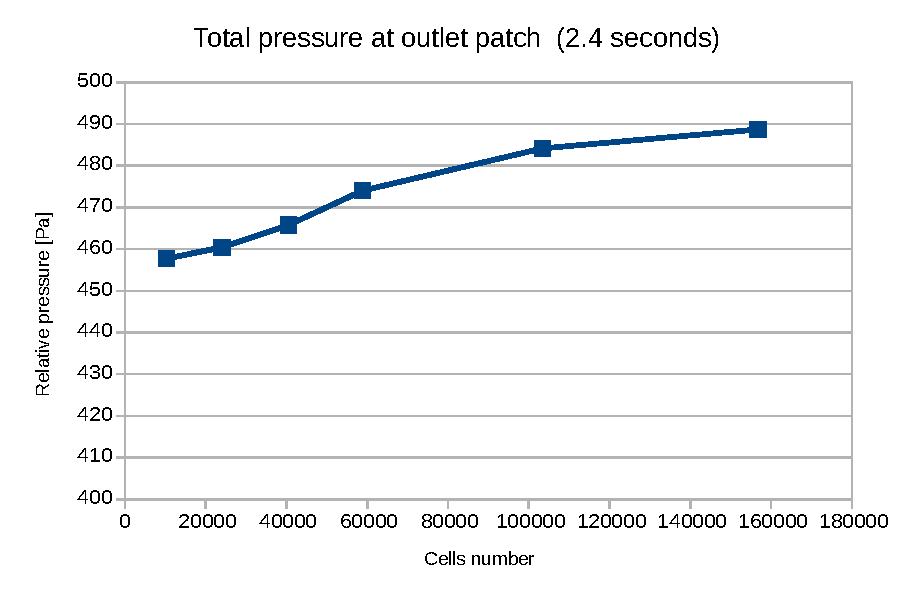
\includegraphics[width=8.5cm]{{images/meshsensitivity/totalpout-2.4-noregion}.pdf}}
\subfigure[Mesh with refinement region]{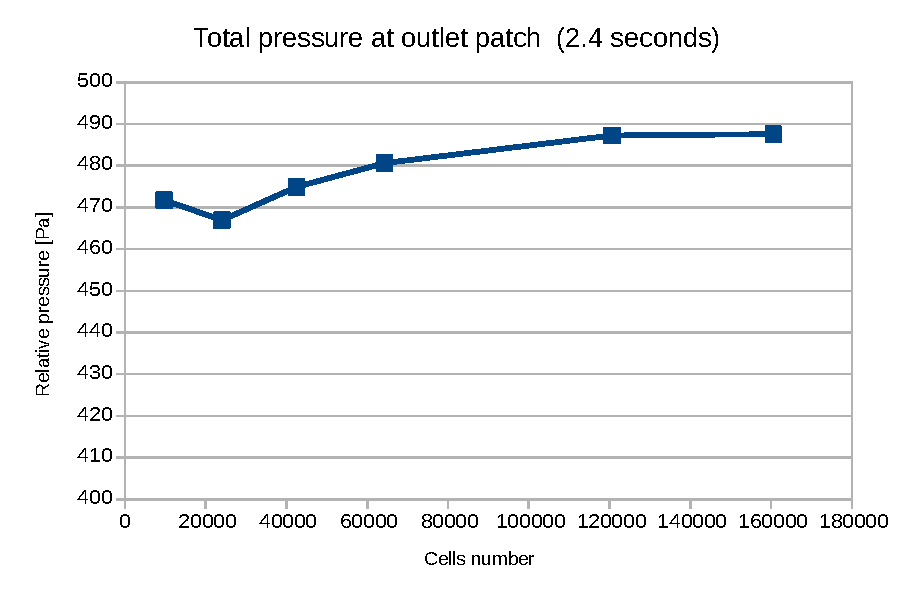
\includegraphics[width=8.5cm]{{images/meshsensitivity/totalpout-2.4-region}.pdf}}
\caption{Total pressure average on outlet patch at 2.4 seconds}
\label{fig:meshsensityvity-totalpressure-case1}
\end{figure}

\begin{figure}[htbp]
\centering
\subfigure[Mesh without refinement region]{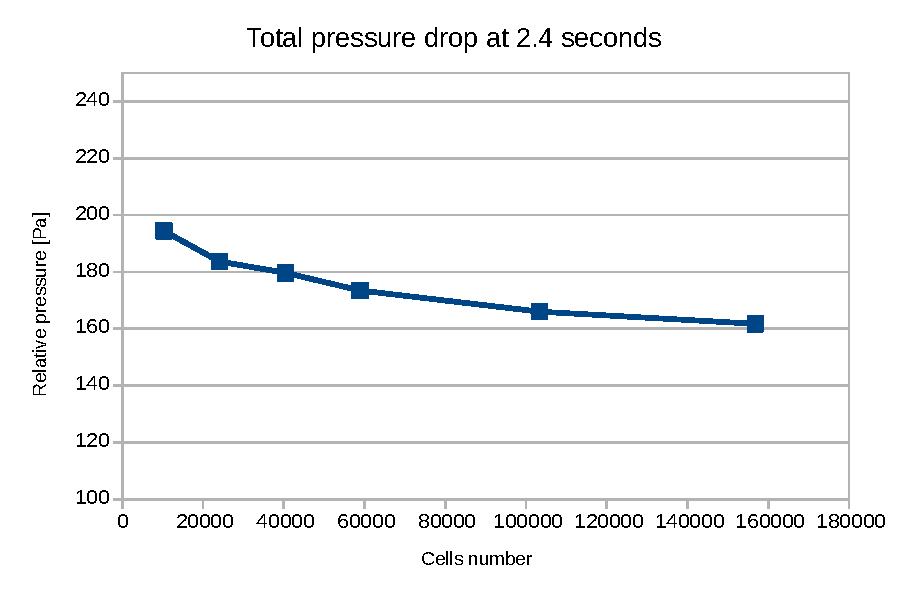
\includegraphics[width=8.5cm]{{images/meshsensitivity/totalpdrop-2.4-noregion}.pdf}}
\subfigure[Mesh with refinement region]{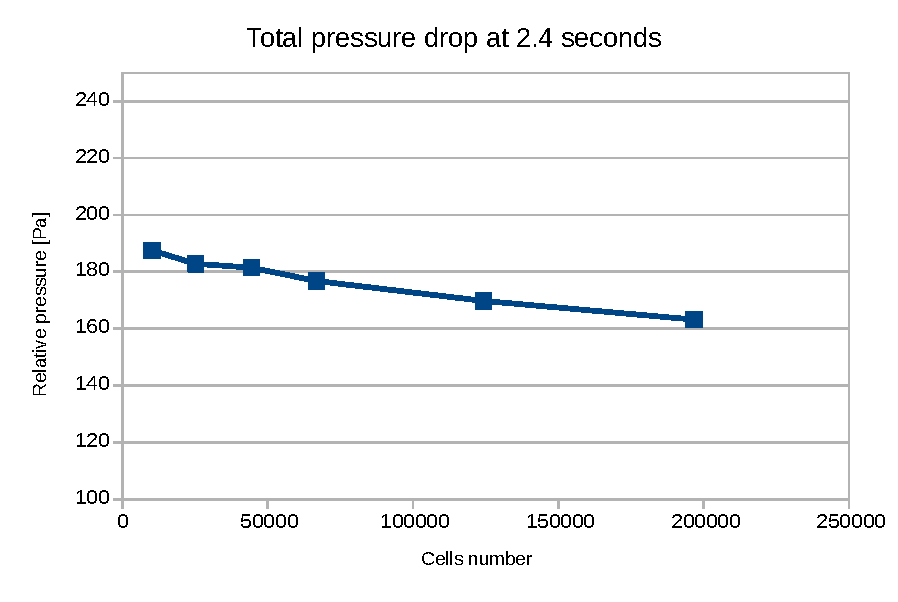
\includegraphics[width=8.5cm]{{images/meshsensitivity/totalpdrop-2.4-region}.pdf}}
\caption{Total pressure drop between inlet and outlet at 2.4 seconds.}
\label{fig:meshsensityvity-totalpressure-case2}
\end{figure}

\begin{figure}[htbp]
\centering
\subfigure[Mesh without refinement region]{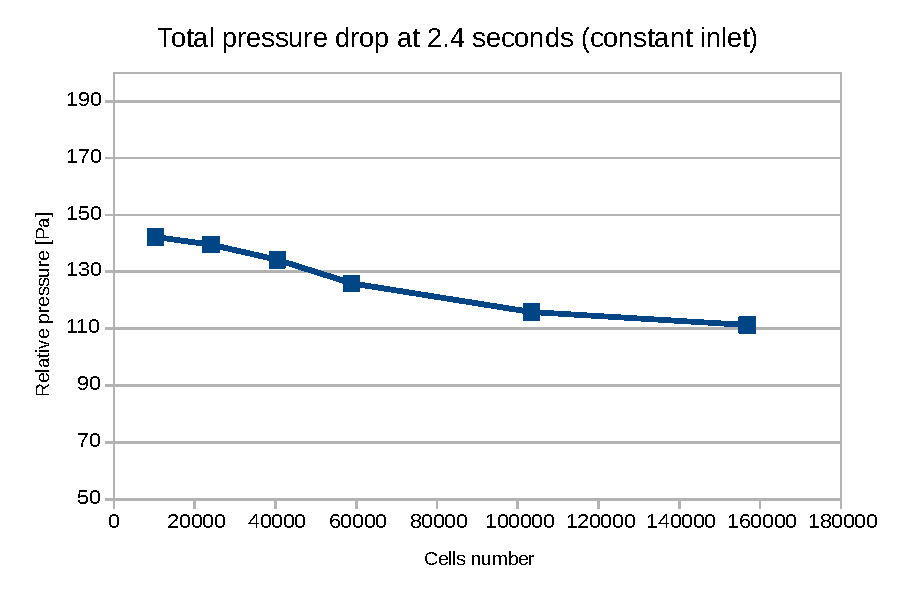
\includegraphics[width=8.5cm]{{images/meshsensitivity/totalpdrop-constantref-noregion}.pdf}}
\subfigure[Mesh with refinement region]{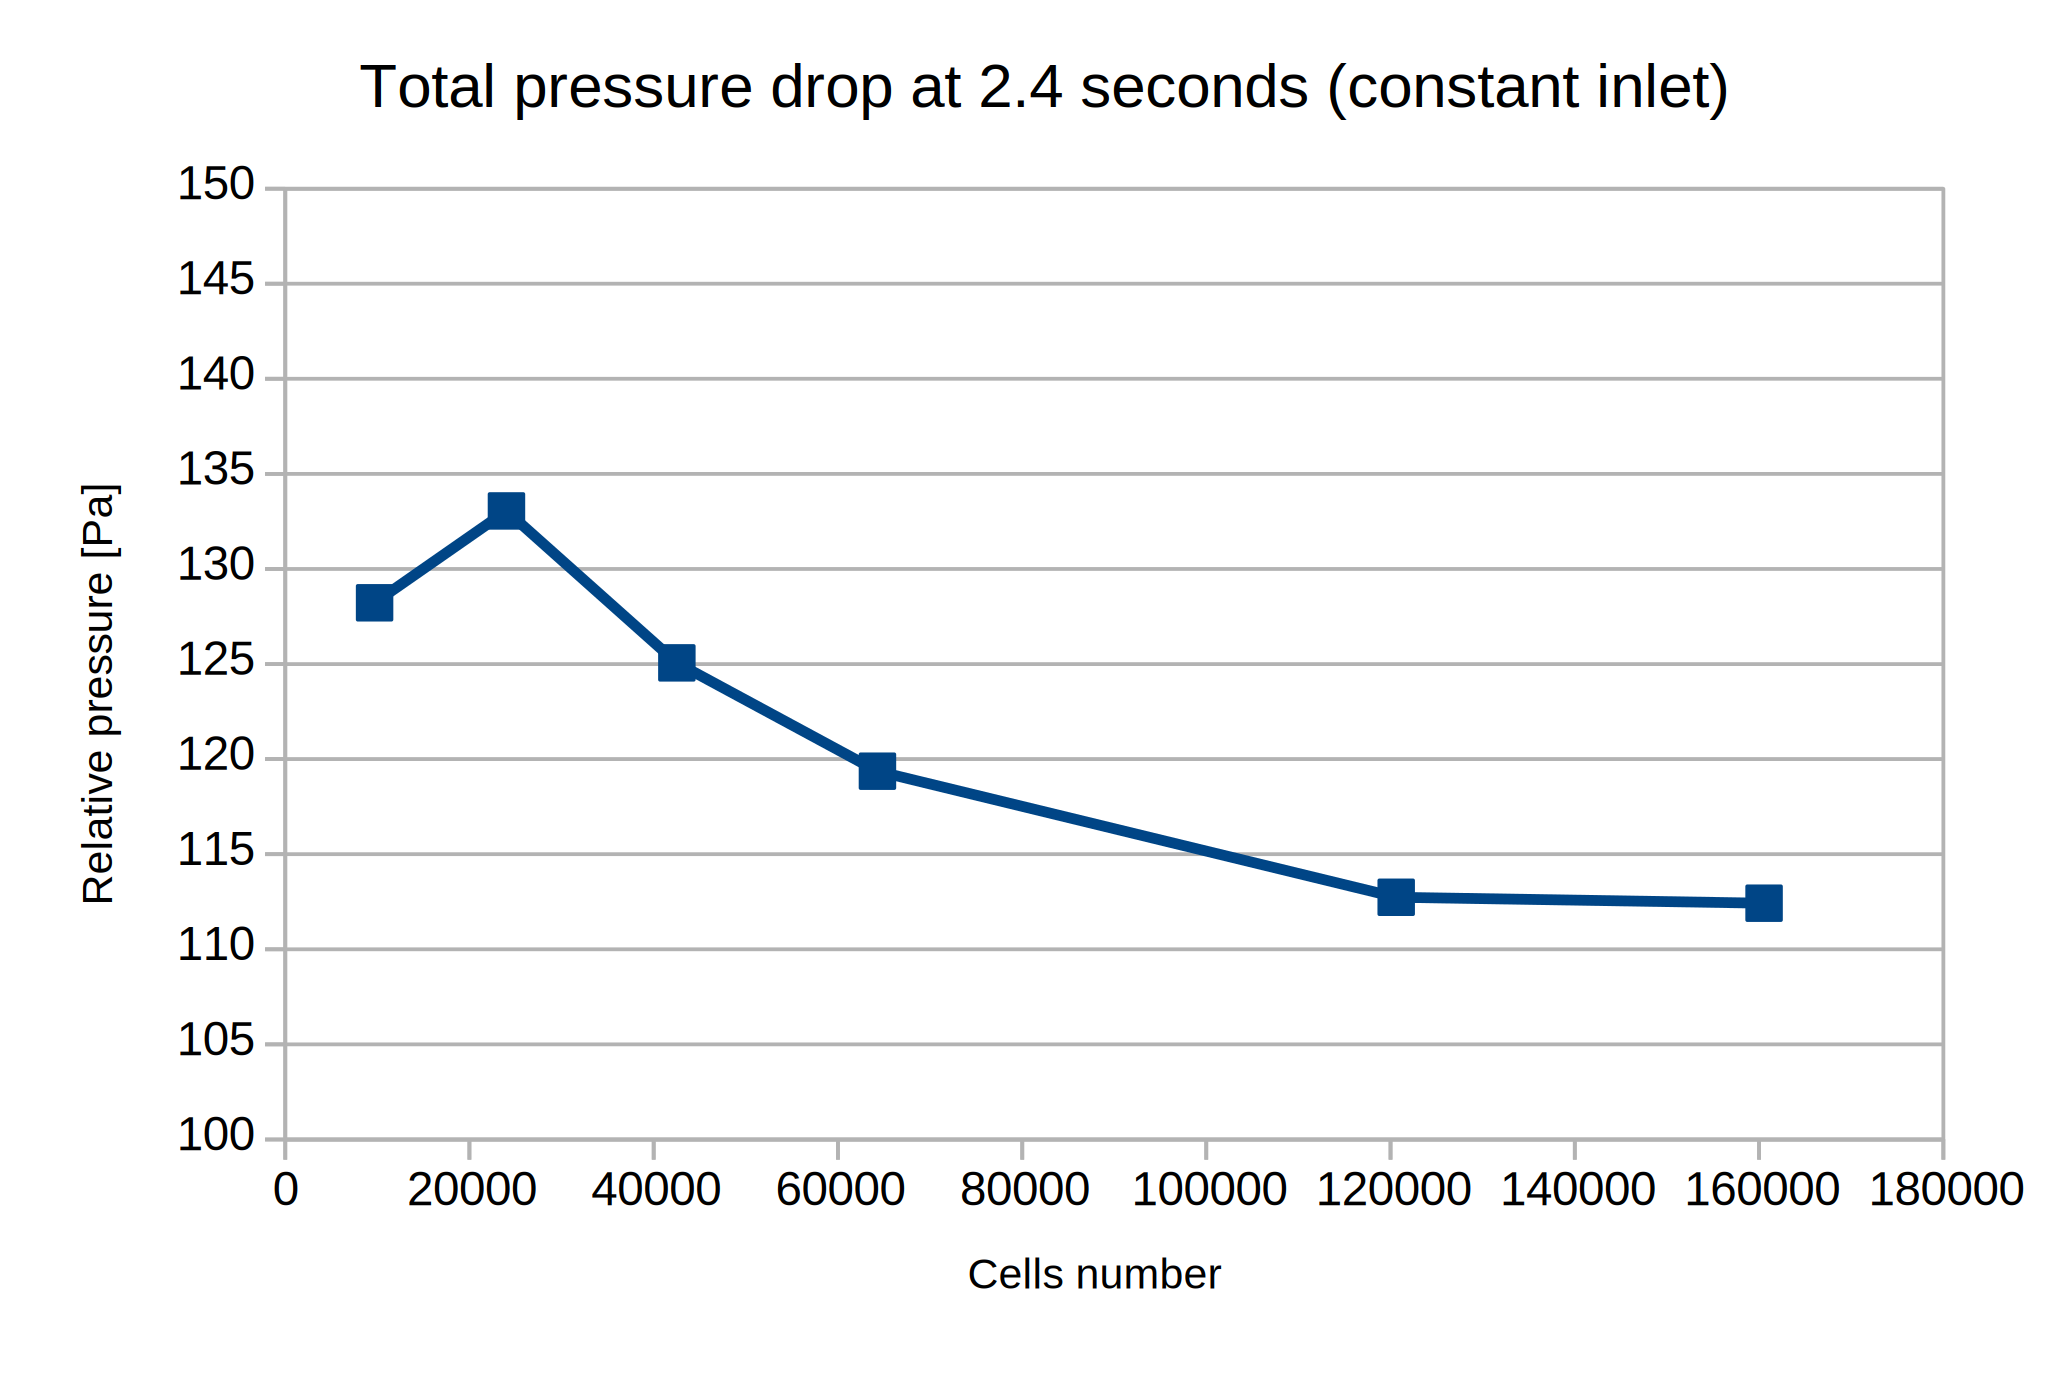
\includegraphics[width=8.5cm]{{images/meshsensitivity/totalpdrop-constantref-region}.pdf}}
\caption{Total pressure drop between reference inlet at 0 seconds and outlet at 2.4 seconds.}
\label{fig:meshsensityvity-totalpressure-case3}
\end{figure}

Some cases shows a great convergence at mesh 120, some others highlight the fact that probably the best possibility is to go towards mesh 160, even though the difference is in general small.

Due to limitation in computational time we stay in the middle between mesh 80 which seems good from the point of view of the power and mesh 160 which seems the best even in any case.

To let us perform more analysis in next chapter and balancing the fact that power shows a good convergence we will chose mesh 120 to perform further simulation if not explicitely specified.

\section{Final mesh}

As we have said before we will design a proper mesh that fits with 120 cells in y direction.
Up to now we have applyed one layer with snappyHexMesh around the blades and then we have splitted it with refineWallLayer four times.
Now the aim is to create the biggest layer as possible with snappy hex mesh, divide that region with a proper number of layer with snappy, and then divide again the last layer with refineWallLayer utility.
\\
We manage to obtain 4 layer with snappyHexMesh and then we apply refineWallLayer 3 further times.

Then we add a refinement region of 3 lever around each blade with an extension of $4 \mm$

We keep 2 layer per region where we have contact between moving surfaces. The total number of layer around Ami patches so will be equal to 4, two per side.

\begin{figure}[hbtp]
\centering
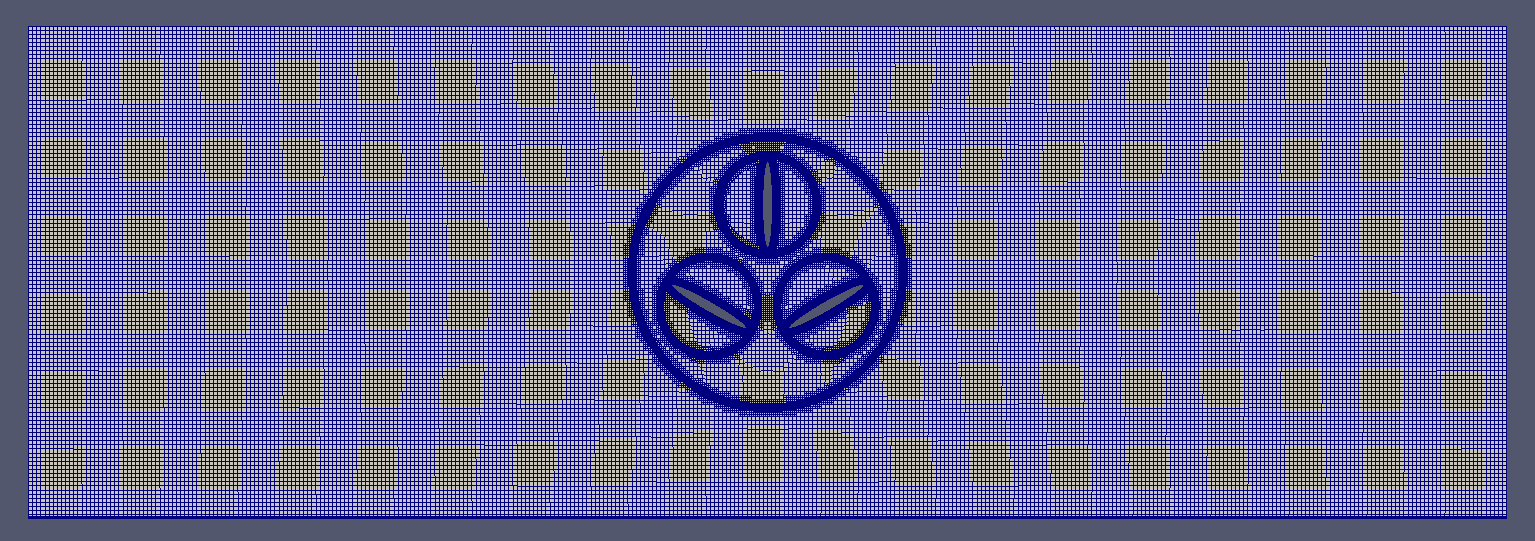
\includegraphics[width=17cm]{images/mesh-120/view-full.png}
\caption{Full view of the mesh}
\end{figure}

\begin{figure}[htbp]
\centering
\subfigure[Blade tip region.]{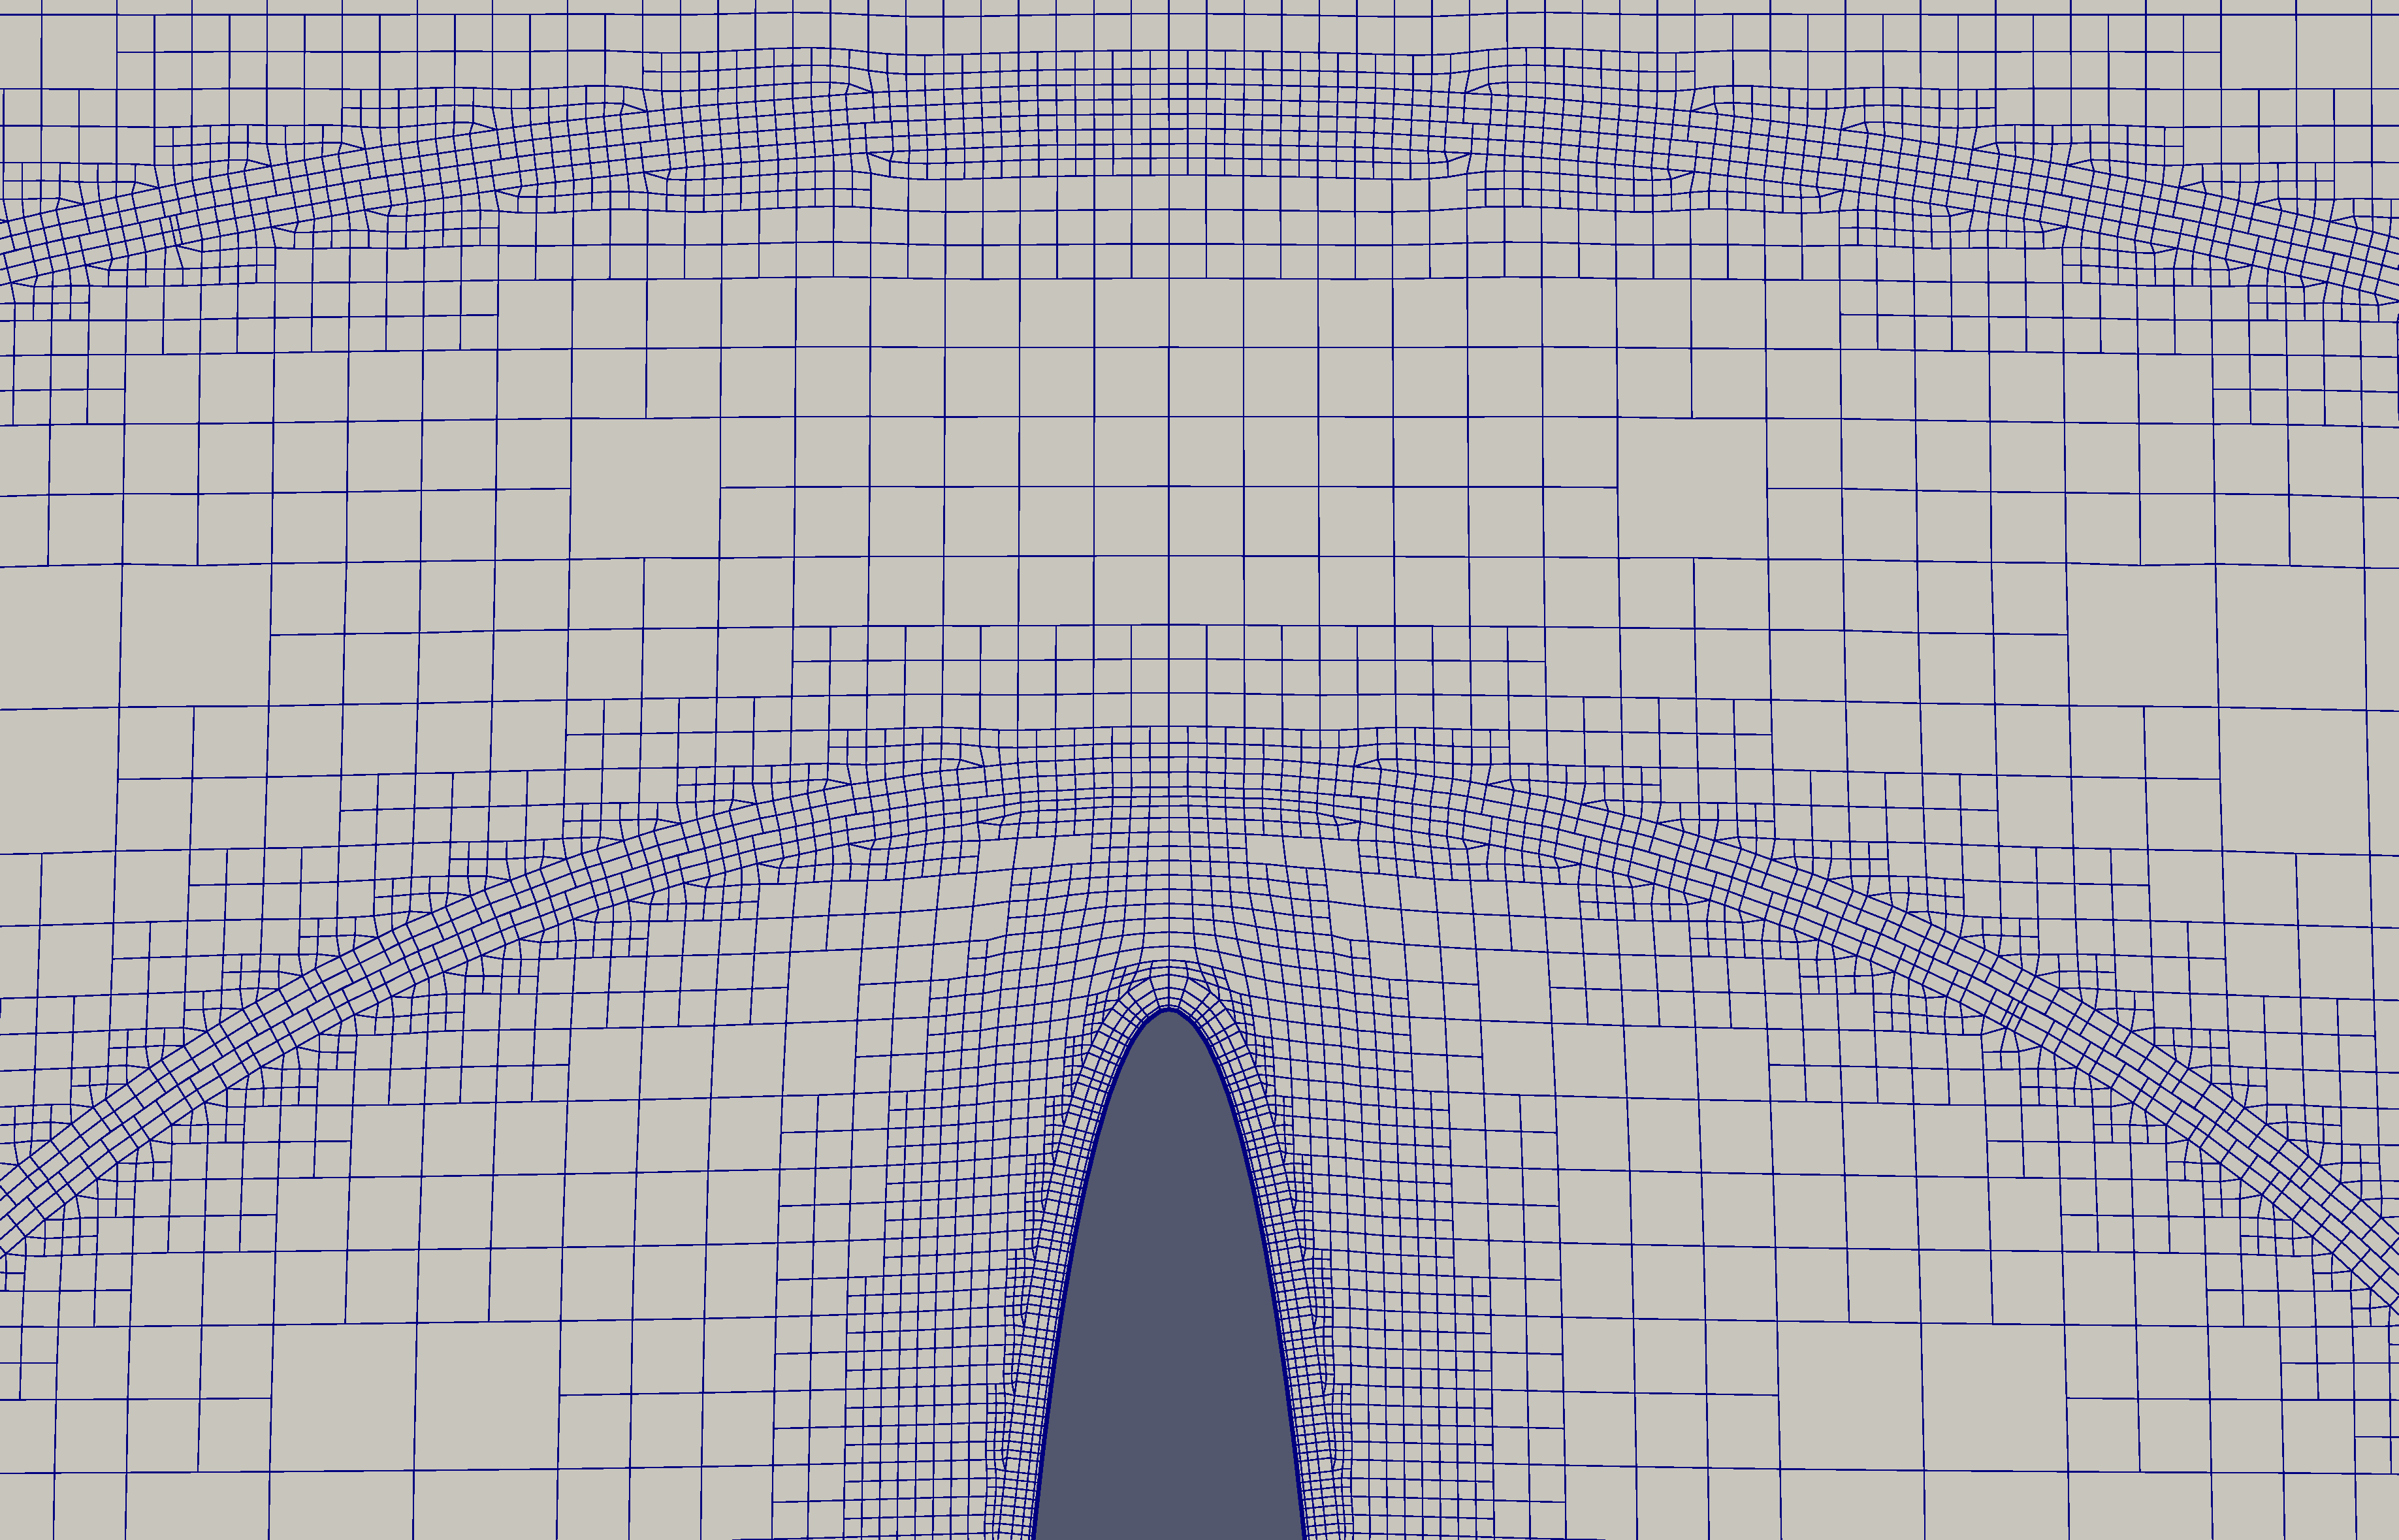
\includegraphics[width=8.5cm]{{images/mesh-120/view-bladetip}.pdf}}
\subfigure[Boundary layer.]{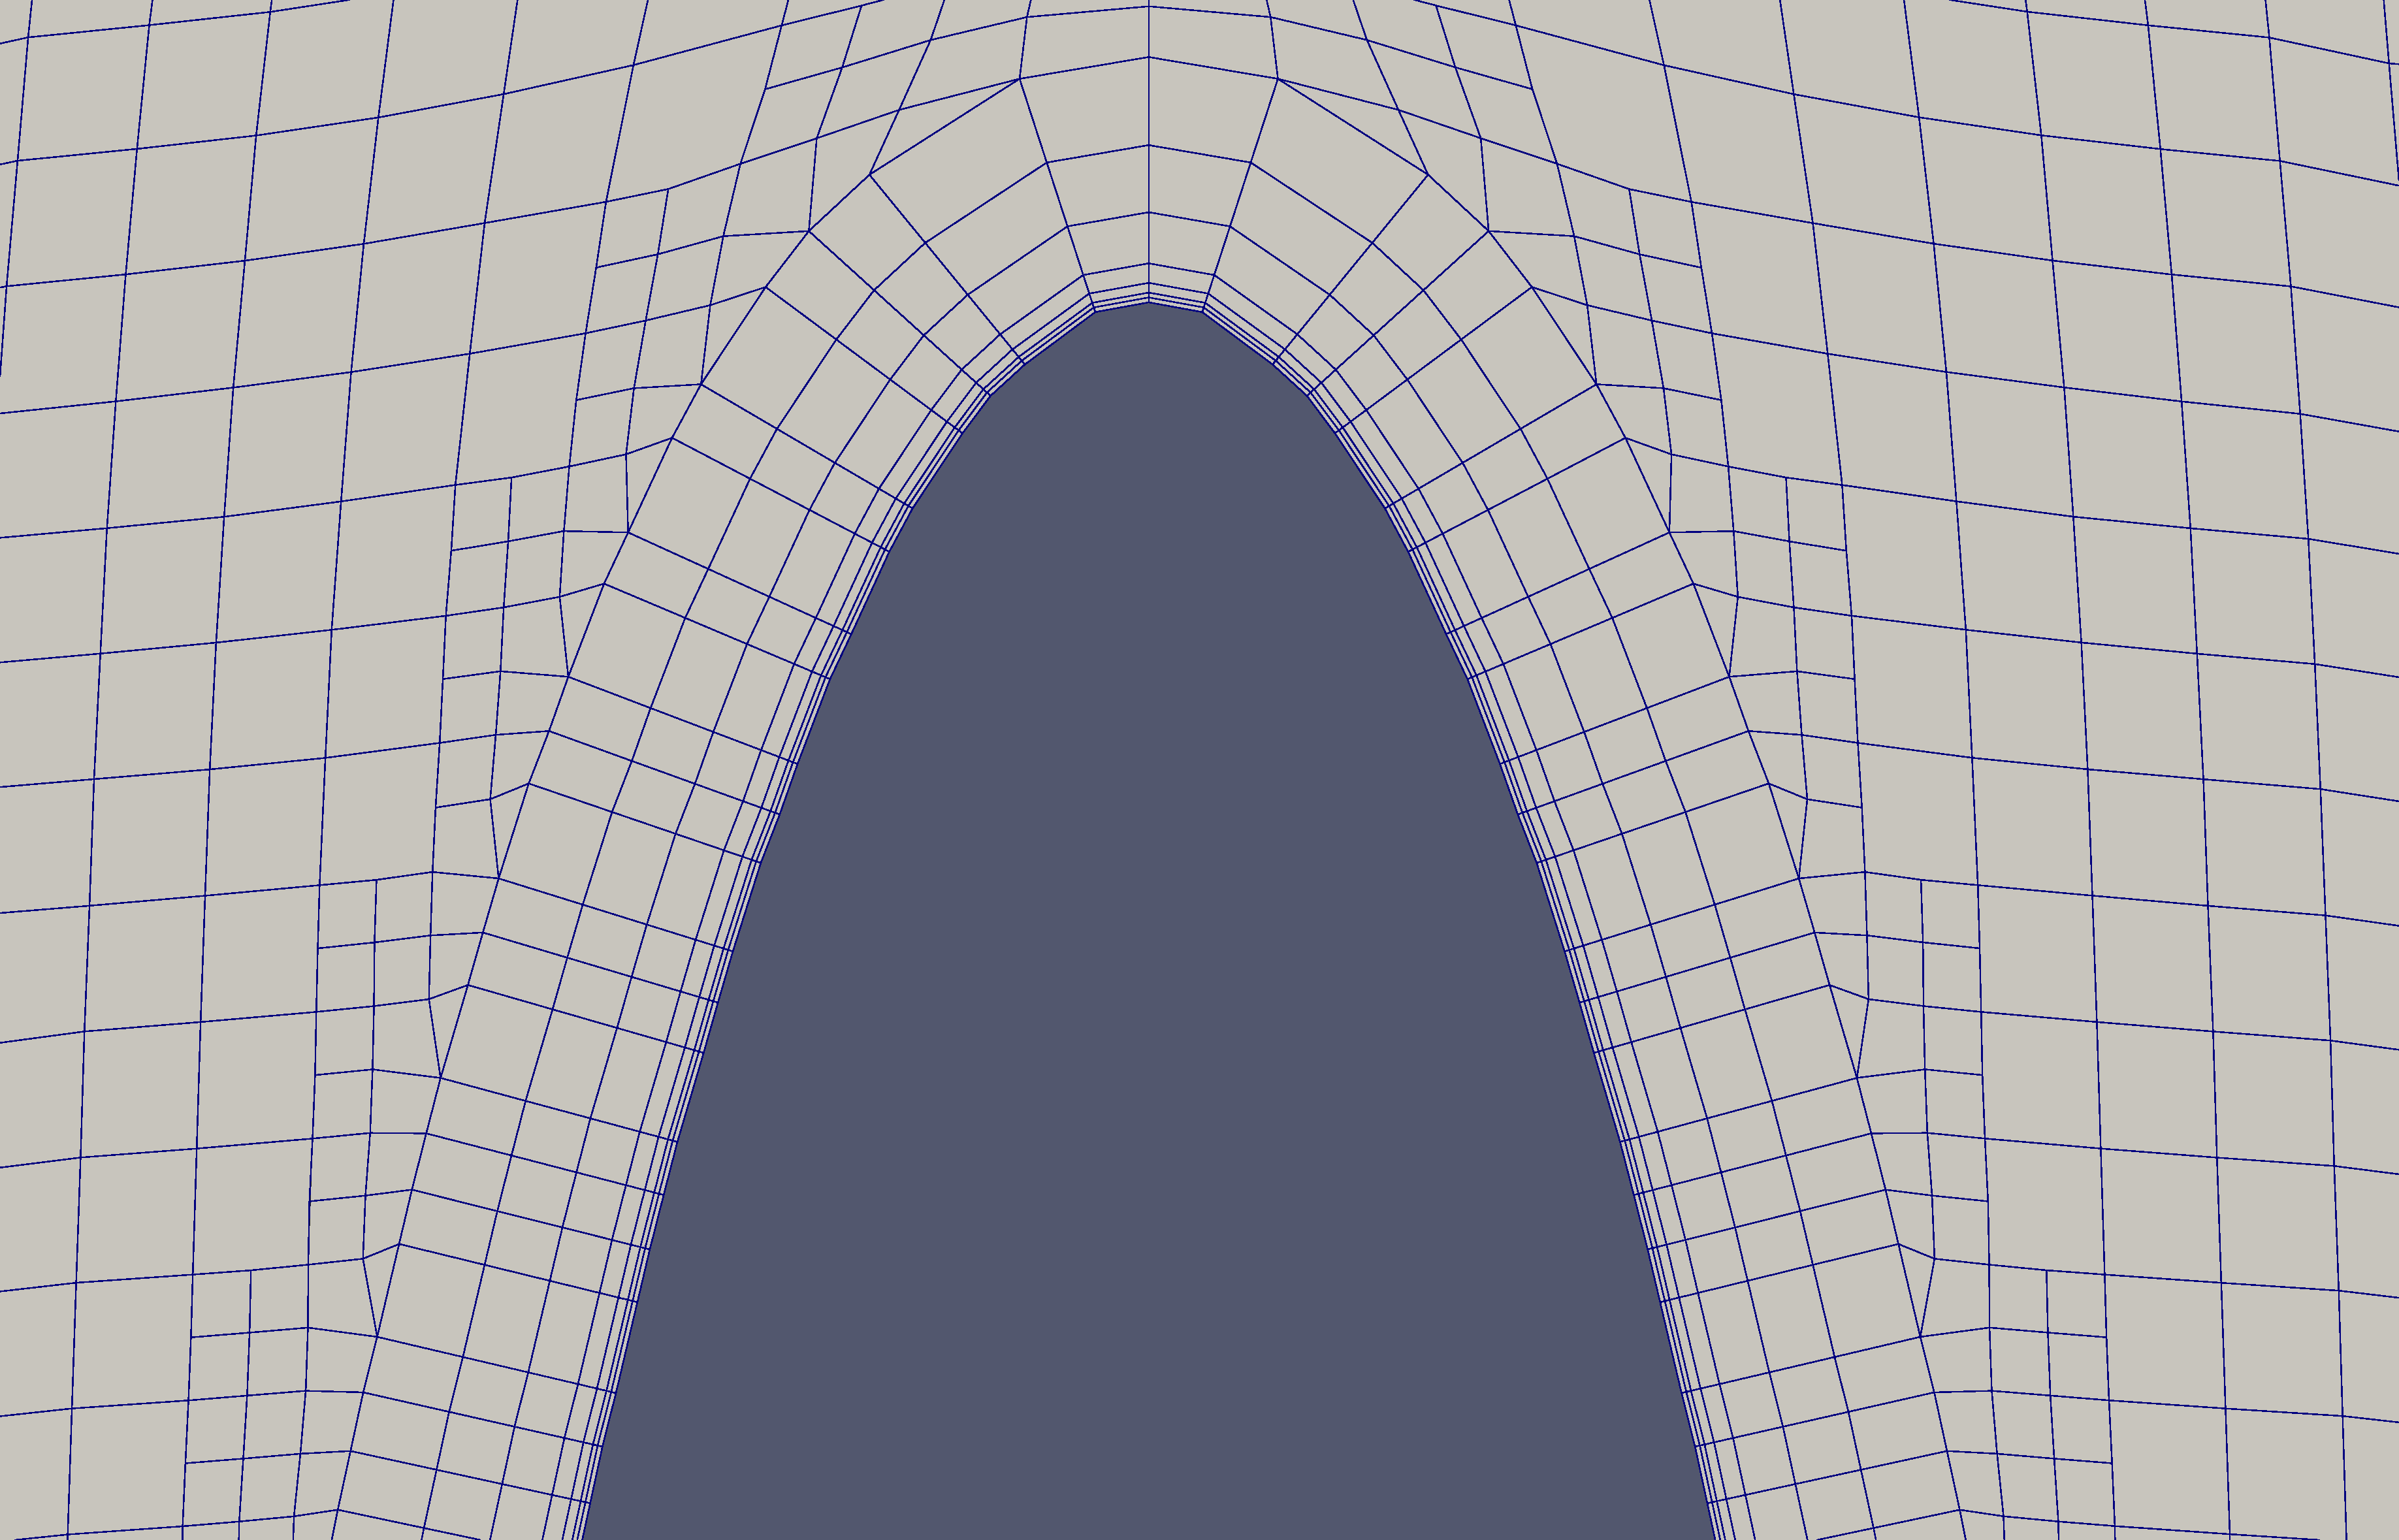
\includegraphics[width=8.5cm]{{images/mesh-120/view-bladetip-zoom}.pdf}}
\end{figure}

\begin{figure}[H]
\centering
\includegraphics[width=17cm]{images/mesh-120/view-blade0.pdf}
\caption{View of the blade 0 at time 0 seconds}
\end{figure}

We finally obtain a mesh whose characteristics are displayed in table \ref{table:mesh120}. All the properties, both that represented and all the others, respect our limits of the mesh quality control. 
\begin{table}[H]
\centering
\caption{Properties of the mesh}
\label{table:mesh120}
\begin{tabular}{lr|c}
\toprule
Cells                 & $113754$     &    \\
Max Skewness          & $2.71645$    & OK \\
Max non-orthogonality & $58.52\,^{\circ}$ & OK \\
Max aspect ratio      & $16.1092$    & OK \\ \bottomrule
\end{tabular}
\end{table} 

\section{Numerical Schemes}

\section{Gravitational influence}

\section{Turbolence}

\subsection{Turbolence model}

\paragraph{Laminar}

\paragraph{$k-\varepsilon$ model}

\paragraph{$k-\omega $ SST model}

\subsection{Turbolence intensity}

\section{The domain's sizes}

\section{Results}

\section{Blade speed ratio Analysis}

From what we have seen in mesh sensitivity analysis, the power is quite accurately computed even for a mesh size smaller that that we consider mesh independent.

To obtain a larger number of points from the blade speed ratio analysis we have decided to run most of the simulation with a mesh with 80 cells in the y direction instead of 120. This reduces the number of cells to around 60000 instead of 110000. 
\\Computational time is in this way reduced, but we risk to have errors with a mesh coarser,

So our idea is to validate just the most significant points with the finer mesh and then compare with the results of the coarser.

We consider that this operating procedure is a proper balance between accuracy and computational cost.

\begin{figure}[hbtp]
\centering
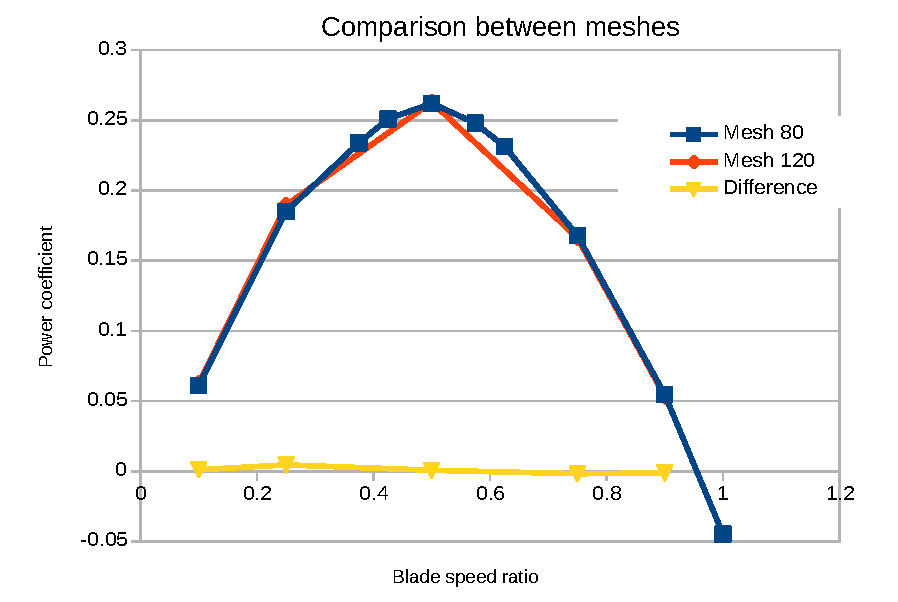
\includegraphics[width=15cm]{images/bsr/bsr-mesh80-120.pdf}
\caption{Comparison between mesh 80 and mesh 120}
\label{fig:bsr-comparison-80-120}
\end{figure}

As we can see in figure \ref{fig:bsr-comparison-80-120} the difference in this case between mesh 80 and mesh 120 in the points in which we have computed bot, is quite small.
Here the corser mesh is perfectly fine to describe the behaviour of this machine relatively to the power coefficient respect to the blade speed ratio.

We have a confirmation that as the mesh sensitivity analysis already highlighted, power is not influenced too much even with this coarser mesh and the difference with the finer mesh is almost negligible.

\subsection{Comparison with experiments}

Before to compare with the experiments we have to explain how we have calculated the power coefficient.
\begin{equation}
c_\text{P} = \dfrac{\text{Actual Power}}{\text{Flow power}}
\end{equation}
Where the actual power is that calculated with the CFD analysis while the flow power is that of a water flux that flow through a reference surface. 
\begin{equation}
\text{P}_\text{flow} 
= \dot{\text{m}}_\text{flow} \cdot \dfrac{v^2_\text{flow}}{2} 
= \rho \, v_\text{flow} \cdot \text{A}_\text{reference} \, \dfrac{v^2_\text{flow}}{2} 
= \rho \, \text{A}_\text{reference} \, \dfrac{v^3_\text{flow}}{2}
\end{equation}

The flow speed is that imposed to the flow and can be found from the blade speed ratio:
\begin{equation}
\text{bsr} = \dfrac{\omega \, r}{v_\text{flow}} \quad \quad \Rightarrow \quad \quad v_\text{flow} = \dfrac{\omega \, r}{\text{bsr} }
\end{equation}

Now we have to define the reference area. We consider it as the total projected surface occupied by the blades during the motion which in formulas becomes:
\begin{equation}
\text{A}_\text{reference} = 2\, \text{R} \cdot t = 0.0396 \msquare
\end{equation}
\begin{conditions}
R & 0.055 + 0.07 / 2 = 0.09 \m  \text{ is distance between the center of rotation and blade tip} \\
t & 0.22 \m \text{ is blade thickness}
\end{conditions}

The results plotted in figure \ref{fig:bsr-comparison-80-120} are then shown in table \ref{table:bsr80}

\begin{table}[]
\centering
\caption{Blade speed ratio results with mesh 80.}
\label{table:bsr80}
\begin{tabular}{ccccc}
\toprule
BSR             & Inlet U $[\ms]$               & $\text{P}_\text{flow} [\w]$     & Power [W]                   & $c_\text{P}$                 \\ \midrule
$\round{0.1}$   & $\round{5.75958653158129}$  & $\round{3783.02414063558}$ & $\round{231.309697474}$  & $\round{0.061144124085642}$  \\
$\round{0.25}$  & $\round{2.30383461263251}$  & $\round{242.113545000677}$ & $\round{44.7832513893}$  & $\round{0.184967971904153}$  \\
$\round{0.375}$ & $\round{1.53588974175501}$  & $\round{71.7373466668673}$ & $\round{16.7771858587}$  & $\round{0.233869617963564}$  \\
$\round{0.425}$ & $\round{1.3551968309603}$   & $\round{49.2801842053078}$ & $\round{12.3603554173}$  & $\round{0.250817962972807}$  \\
$\round{0.5}$   & $\round{1.15191730631626}$  & $\round{30.2641931250846}$ & $\round{7.93038993609}$  & $\round{0.262038703735235}$  \\
$\round{0.575}$ & $\round{1.0016672228837}$   & $\round{19.8991982411997}$ & $\round{4.93294852137}$  & $\round{0.247896847982384}$  \\
$\round{0.625}$ & $\round{0.921533845053006}$ & $\round{15.4952668800433}$ & $\round{3.58593868415}$  & $\round{0.231421550329566}$  \\
$\round{0.75}$  & $\round{0.767944870877505}$ & $\round{8.96716833335841}$ & $\round{1.50671756951}$  & $\round{0.168026015961462}$  \\
$\round{0.9}$   & $\round{0.639954059064587}$ & $\round{5.18933352624908}$ & $\round{0.2842517898}$   & $\round{0.05477616506285}$   \\
$\round{1}$     & $\round{0.575958653158129}$ & $\round{3.78302414063558}$ & $\round{-0.16891080726}$ & $\round{-0.044649677342958}$ \\ \bottomrule
\end{tabular}
\end{table}

Finally we are able to compare the results to the real experiments.
\\
The results are shown in figure \ref{fig:bsr-comparison-exp}

\begin{figure}[hbtp]
\centering
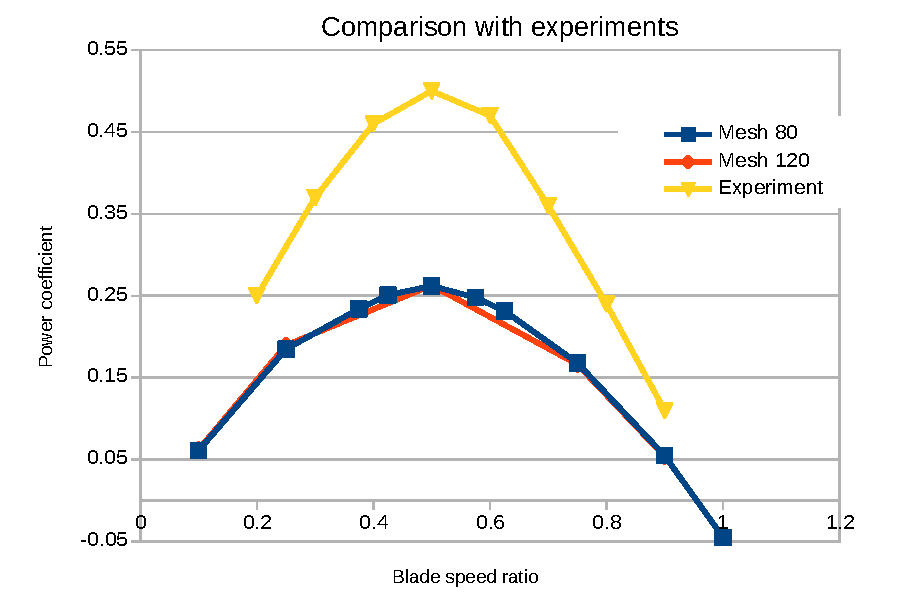
\includegraphics[width=15cm]{images/bsr/bsr-exp.pdf}
\caption{Comparison between mesh 80 mesh 120 and experimental results}
\label{fig:bsr-comparison-exp}
\end{figure}

As we immediatly see, the trend it quite well described, but the calculate absolute value is around half of the value obtainerd through experiments.

It seems like we have considered a different reference area respect to the experiments.

Howether we will show an adimensionalized comparison to at least reveal is the trend (radio of calculated power at two different blade speed ratio is coherent).
In figure \ref{fig:bsr-comparison-exp-relative} we can see the two data set normalized respect to their maximum value.
In this case the complice with experimental results is much better, and it seems to have a physical meaning, in particular for values of $c_\text{P}$ greter than 0.5.

\begin{figure}[hbtp]
\centering
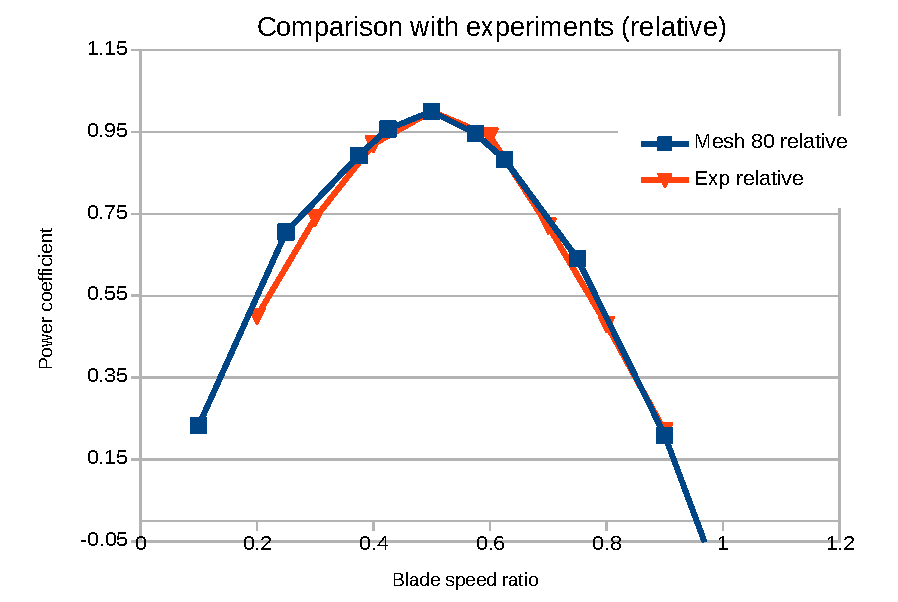
\includegraphics[width=15cm]{images/bsr/bsr-exp-relative.pdf}
\caption{Relative comparison between mesh 80 and experimental results}
\label{fig:bsr-comparison-exp-relative}
\end{figure}

\section{Conclusion}


















\end{document}